% \noindent 
% \textcolor{blue}{
% The content of this section will be dependent on the interests of contributors and what they want to write about.
% }
In this section, we aim to give an overview of technologies and techniques for building fast ML algorithms. 
This requires {\it codesign}: building algorithms with hardware in mind and providing efficient platforms for programming the hardware.  Section~\ref{sec:deploy} and Section~\ref{sec:train} focus on neural network design and training for efficient implementation in hardware. 
In Section~\ref{sec:cmos} and Section~\ref{sec:beyondcmos}, we classify our discussion of ML hardware compute platforms into two categories: ``Conventional CMOS Hardware'' and ``Emerging Beyond CMOS Hardware.''  
The former will address nearer-term hardware solutions, while the latter will focus on the speculative end of the spectrum. Meanwhile, because the area of programming new hardware is rapidly moving, we lay out an example of the options and challenges for one device family: FPGAs. 
This is presented in Sec.~\ref{sec:codesign}, and from the details for FPGAs we hope the reader also gets a sense of the fundamental approaches for designing software for emerging hardware.   


\subsection{Systematic Methods for the Efficient Deployment of ML Models}
\label{sec:deploy}

As discussed in Section~\ref{sec:apps}, many ML problems in science
require low latency, often with
constrained resources. However, most of the current state-of-the-art NN models have prohibitively high latency with a large
memory footprint and energy consumption. 
For this reason, practitioners have been forced to use sub-optimal models (e.g. shallow NNs)
with non-ideal accuracy to avoid this latency problem.
There is a large body of literature that has
focused on solving this problem by making NN models more efficient
(in terms of latency, memory footprint and energy consumption). These efforts could be broadly categorized as follows:
(i) Designing new efficient NN architectures;
(ii) NN and hardware co-design;
(iii) Quantization (low precision inference);
(iv) Pruning and sparse inference; and
(v) Knowledge distillation.
Here we briefly discuss each of these approaches.


% --------------------------------------------------------------------------------
\paragraph*{Designing new efficient NN architectures}
One line of research has been focused on finding new NN models
that are efficient by design. A notable early work is SqueezeNet~\cite{iandola2016squeezenet},
a new NN model without any expensive Fully Connected layers,
along with a new lightweight \emph{Fire module}, that resulted
in a $50\times$ smaller model as compared to AlexNet, but with the
same accuracy. Later on several new innovations were made in
efficient NN architecture design.
One focus has been to find efficient layers/operators.
Notable works are
group convolutions~\cite{ioannou2017deep}, 
depthwise convolutions~\cite{howard2017mobilenets},
spatial separable convolutions~\cite{mamalet2012simplifying},
shuffle layers~\cite{ma2018shufflenet},
and shift convolutions~\cite{wu2018shift}, to name a few.

Another focus has been to find similar substitutes to \emph{Fire module} that are more efficient and result in better
accuracy/generalization. Notable works include
residual networks~\cite{he2016deep} (originally designed
to solve issues with vanishing gradients, but these structure are generally more efficient
than non-residual architectures), densely connected networks~\cite{huang2017densely},
squeeze-and-excite modules~\cite{hu2018squeeze},
and inverted residual blocks~\cite{sandler2018mobilenetv2}.

These classical techniques mostly found new architecture modules
through a manual design search. 
This is not scalable, and as such recent approaches have proposed automated methods that use neural architecture search (NAS). 
NAS methods automatically find the right NN architecture for a given constraint
of model size, depth/width, and/or latency.
The high level approach here is to train a probabilistic \emph{SuperNet}
that includes all possible combinations of NN architectures within the prescribed
constraints, but with learnable probabilities. 
After this SuperNet is trained, one can sample an architecture from its learned probability distribution.
Notable works include RL based methods~\cite{zoph2016neural}, efficient NAS~\cite{pham2018efficient}, MNasNet~\cite{tan2019mnasnet}, DARTS~\cite{liu2018darts}, and Differentiable NAS~\cite{wu2019fbnet}.

% \begin{outline}
%     \1 SqueezeNet ~\cite{iandola2016squeezenet};
%     \1 MobileNet family~\cite{howard2017mobilenets,sandler2018mobilenetv2,howard2019searchin}
%     \1 ShuffleNet~\cite{ma2018shufflenet}, ShiftNet~\cite{wu2018shift}, DenseNet~\cite{huang2017densely}
%     \1 EfficientNet~\cite{tan2019efficientnet}
%     \1 Discuss the methodology of AutoML/DNAS and how it works
% \end{outline}

% --------------------------------------------------------------------------------
\paragraph*{NN and hardware co-design}
Another promising line of work has been to tailor the NN architecture for a specific hardware
platform, and/or co-design them together. This is quite promising for
configurable hardware such as FPGAs. The importance of hardware-aware NN design is that
the cost of performing different types of operations varies for different hardware.
For example, a hardware that has a dedicated cache hierarchy can execute bandwidth
bound operations much more efficiently than a hardware without a cache hierarchy.
Notable works in this area include SqueezeNext~\cite{gholami2018squeezenext}, where both the NN and the hardware
accelerator were co-designed with a manual tuning approach.
More recent works have proposed to automate hardware-aware design
through NAS.
Notable works include ProxylessNAS~\cite{cai2018proxylessnas}, OnceForAll~\cite{cai2019once}, FBNet~\cite{wu2019fbnet},
and MobileNetV3~\cite{howard2019searching}.

% --------------------------------------------------------------------------------
\paragraph*{Quantization (low precision inference)}
A common solution is to compress NN models with quantization~\cite{asanovic1991experimental, hubara2016binarized, rastegari2016xnor, zhou2017incremental, zhou2016dorefa, cai2017deep, jacob2018quantization, zhang2018lq, choi2018pact, wang2019haq, dong2019hawq, chin2020one, cai2020zeroq, gholami2021survey},
where low bit-precision is used for weights/activations.
A notable work here is Deep Compression~\cite{han2015deep}, which used
quantization to compress the model footprint of the
SqueezeNet model discussed above, bringing its size to 500x smaller than AlexNet. 
In quantization, the model size is reduced without changing the original network architecture,
and it could potentially permit the use of low-precision matrix multiplication or convolution. Therefore, both the memory footprint
and the latency could be improved.

The quantization methods can be broadly classified into two categories of \emph{Post-Training Quantization} (PTQ),
and \emph{Quantization-Aware Training} (QAT). In PTQ, a pre-trained model in single precision is quantized to low precision
without any fine-tuning or re-training~\cite{banner2018post,meller2019same,choukroun2019low,zhao2019improving,fang2020post,fang2020near,lee2018quantization,nagel2019data,cai2020zeroq,hawks2021ps}. As such, these quantization methods are typically very fast, and, in some cases, do not even require any training data~\cite{cai2020zeroq, haroush2020knowledge,nagel2019data}.
However, PTQ often leads to high accuracy degradation especially for low precision quantization.
To address this, some quantization methods adopt QAT to re-train the model after the quantization, so that the parameters can
get adjusted. 
This approach often results in higher accuracy, but at the cost of longer
time associated with re-training the model~\cite{courbariaux2015binaryconnect,lin2015neural,hubara2016binarized,rastegari2016xnor,zhou2016dorefa,zhu2016trained,cai2017deep,hou2016loss,gysel2018ristretto,huang2021codenet,zhou2018explicit}.

Another differentiator is the use of \emph{simulated quantization} (aka fake quantization), versus \emph{integer-only} quantization~\cite{jacob2018quantization,yao2020hawqv3,kim2021bert,lin2016fixed}. In the former, 
the weights/activations are stored in low precision, but they are cast to higher precision during
inference. In the latter, there is no casting involved, and the multiplication and accumulation also happens
in low precision. Using integer-only quantization has the advantage that one can speed up
inference by using low-precision logic for multiplication and addition, besides reducing the memory footprint of the model.

% For some cases, it is possible to map a simulated quantization graph to low precision
% multipliers. However, this could lead to discrepancy which can become large, especially for low precision quantization~\cite{yao2020hawqv3}.

Another distinction is \emph{hardware-aware quantization}. 
Similar to NN architecture design, quantization can also be tailored for specific hardware platforms.
This becomes important for mixed-precision quantization~\cite{zhou2018adaptive, wang2018haq, wu2018mixed, hawq, shen2020q, hawqv2, dong2021hao, yao2020hawqv3}.
The reason is that certain operations in the NN model may benefit more from low precision
quantization than others, based on whether they are bandwidth bound or compute bound.
As such, as schematically
illustrated in Figure~\ref{fig:pruning_quantization},
one must determine the best precision setting based on the tradeoff between the potential footprint/latency gain and the sensitivity to accuracy degradation.

% ----------------------------------------------------------
\begin{figure*}
\centering
% 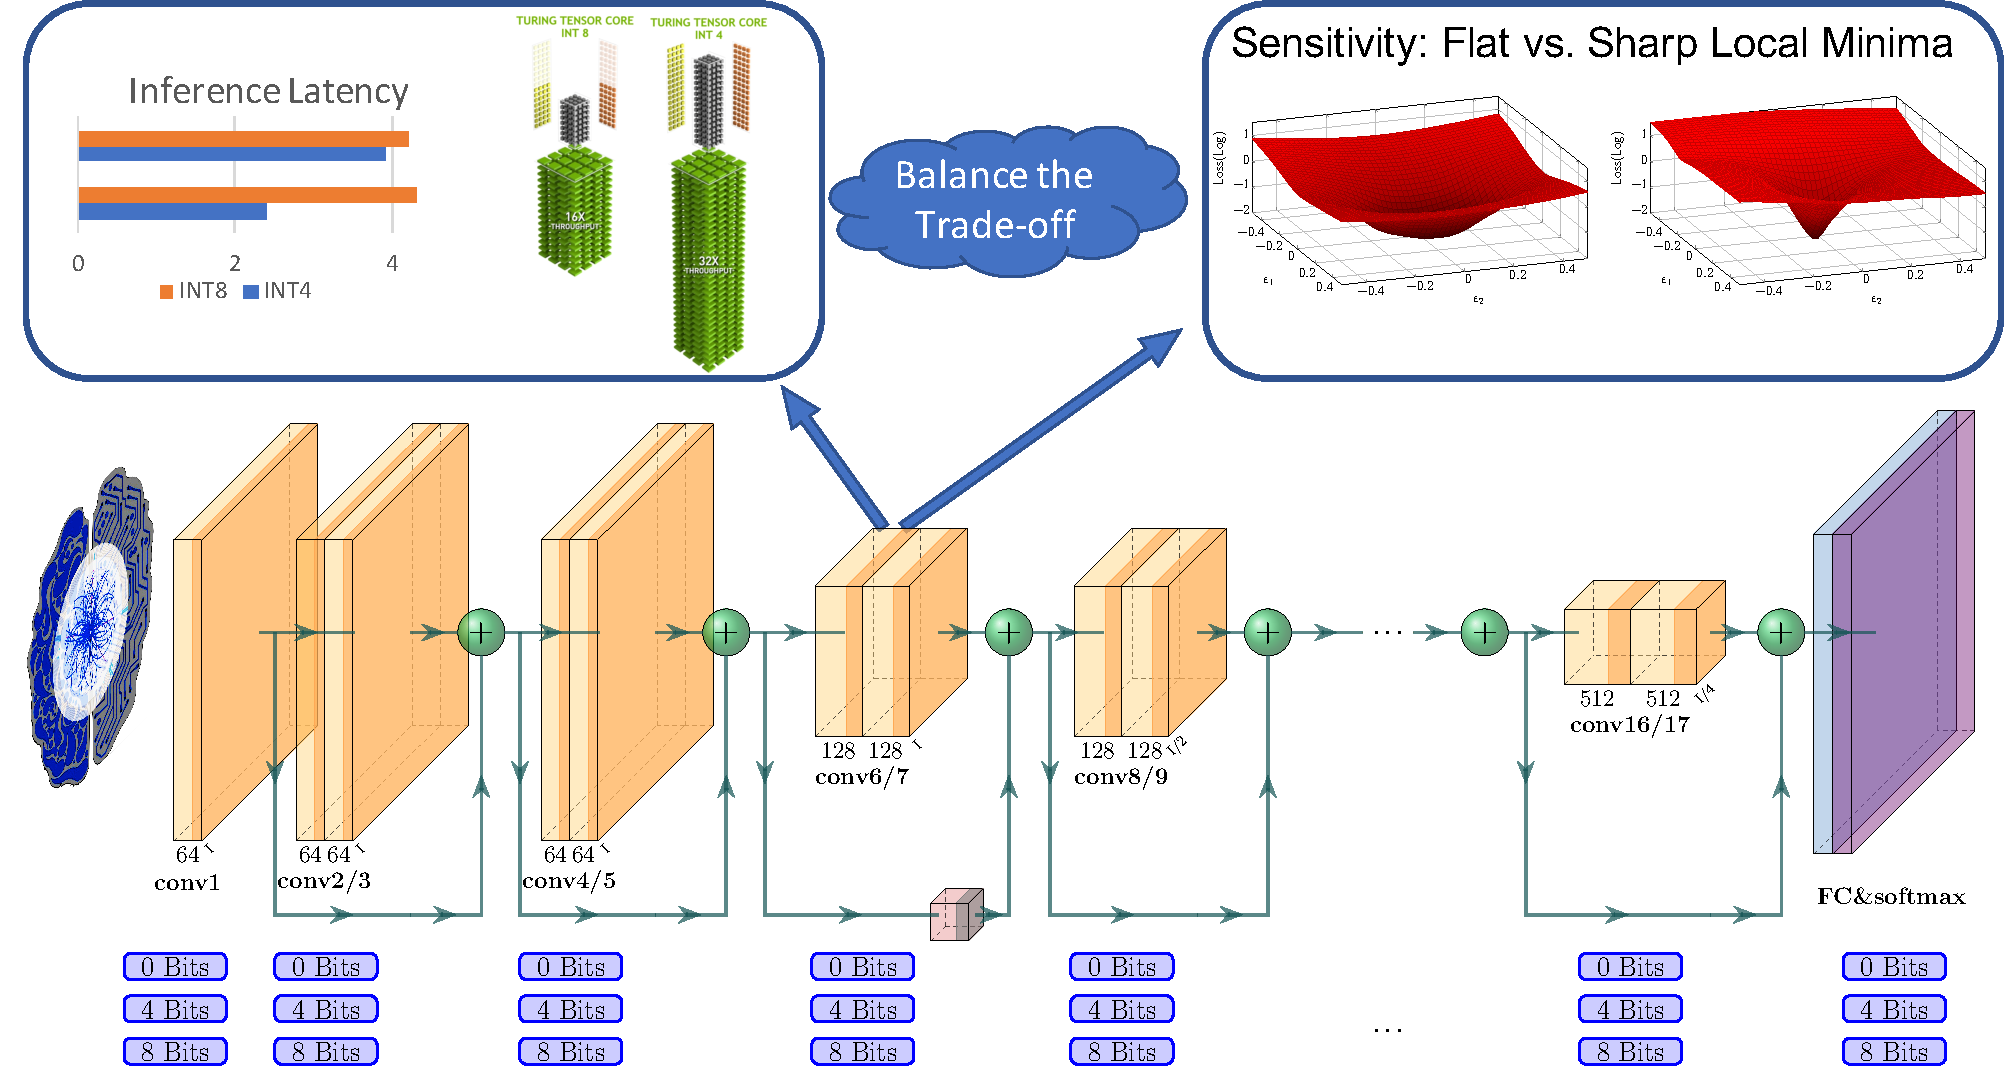
\includegraphics[width=0.8\linewidth]{figures/pruning_quantization_illustration.pdf}
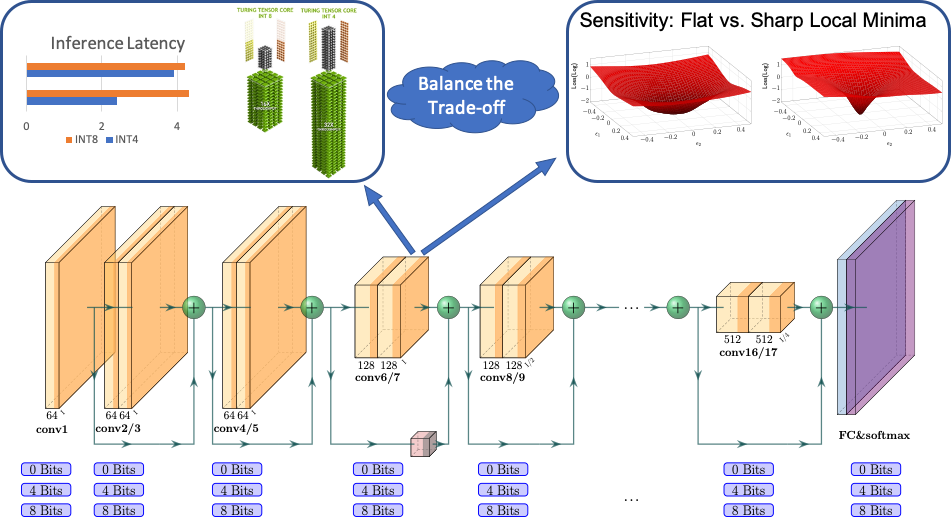
\includegraphics[width=0.8\linewidth]{figures/pruning_quantization_illustration_nologo.png}
\caption{The illustration of hardware-aware quantization and pruning. 
A given NN model can be compressed by using low precision quantization instead
of single precision. The extreme case is to use 0-bit quantization which is 
equivalent to removing/pruning the corresponding neurons.
The goal of compression is to find the best bit-precision setting for
quantization/pruning to reduce model footprint/latency on a target hardware
with minimal generalization loss.
}
\label{fig:pruning_quantization}
\end{figure*}
% ----------------------------------------------------------

% --------------------------------------------------------------------------------
\paragraph*{Pruning and sparse inference}

Another approach to reduce the memory footprint and computational cost of NNs is to apply
pruning, which could be thought of as quantization to 0-bits. In pruning, neurons with small \emph{saliency} (sensitivity) are removed, which results in a sparse computational graph~\cite{lecun1990optimal}. 
Here, neurons with small saliency are those whose removal should minimally affect the model output/loss function.
Pruning methods can be broadly categorized into unstructured pruning~\cite{lecun1990optimal,hassibi1993second,dong2017learning, lee2018snip, xiao2019autoprune, park2020lookahead}, and structured pruning~\cite{luo2017thinet, he2018amc, yu2018nisp, lin2018accelerating, huang2018data, zhao2019variational}.
Unstructured pruning removes neurons without any structure.
With this approach, one can remove most of the NN parameters with little impact on the
generalization performance of the model.
However, this approach leads to sparse matrix operations which are hard to accelerate 
and are typically memory-bounded~\cite{buluc2008challenges,gale2019state,hoefler2021sparsity,blalock2020state}.
This can be addressed with structured pruning, where a
group of parameters (e.g., an output channel) is removed. However, the challenge here is that high degrees of structured
pruning often leads to significant accuracy degradation.

In both approaches, the key question is to find which parameters to prune.
A simple and popular approach is magnitude-based pruning~\cite{chauvin1989back,hanson1988comparing,mozer1988skeletonization,li2016pruning,he2017channel,liu2017learning,he2019filter,lin2020hrank}.
In this approach, the magnitude of parameters is used as the pruning metric.
The assumption here is that small parameters are not important and can be removed.

An important problem with magnitude-based pruning methods is that parameters with small magnitudes can actually be quite sensitive.
It is easy to see this through a second-order Taylor series expansion, where the perturbation is dependent on not just the weight magnitude but
also the Hessian~\cite{lecun1990optimal}. As such there are several works that use
second-order based pruning~\cite{lecun1990optimal,hassibi1993optimal,hassibi1993second,wang2019eigendamage,yu2021hessian}.

Finally, we should mention that it is possible to 
combine pruning and quantization together to compress the NN model.
In fact, pruning could be viewed as quantization to 0-bits. The recent work
of ~\cite{hawks2021ps} proposes a quantization-aware pruning
method and applies to high energy physics problems;  It reports
better results than pruning or quantization alone.

% \begin{outline}
% \1 \textbf{Pruning}~\cite{han2016deep, hassibi1993second, optimalbraindamage, dong2017learning} removes unnecessary nodes/edges from the model for inference. These edges 
%     may be important for training the model, but can be removed without hurting
%     generalization for inference.
%     \2 Current challenges:
%         \3 Pruning beyond 50\% typically results in significant accuracy degradation
%         \3 Need to explore coupled pruning and quantization
%         \3 Unstructured pruning has high generalization but inefficient for HW deployment. Need to study new methods for unstructured pruning that can be deployed efficiently.
% \end{outline}
% --------------------------------------------------------------------------------

\paragraph*{Knowledge distillation}
\textcolor{red}{[S.H. This section is really confusing - needs more meat, and a better explanation] Model distillation~\cite{romero2014fitnets, hinton2015distilling, mishra2017apprentice, li2017learning, yim2017gift, polino2018model, ahn2019variational, yin2020dreaming} trains a large model and then uses it as a teacher to train a compact model. Instead of using class labels during the training of the student model, the key idea of model distillation is to leverage the soft probabilities produced by the teacher, 
which can guide/help the student training. }
% As an example in crystal structure recognition, for an input lattice with the label \textit{Fluorite structure}, classes such as \textit{Antifluorite structure} can also have high probabilities according to the teacher model. Teaching the compact student model to distinguish \textit{Antifluorite structure} (in addition to \textit{Fluorite structure}) from other irrelevant classes can lead to potential performance improvement.

Previous methods of knowledge distillation focus on exploring different knowledge sources. Refs.~\cite{hinton2015distilling, li2017learning, park2019relational} use logits (the soft probabilities) as the source of knowledge, while Refs.~\cite{romero2014fitnets, yim2017gift, ahn2019variational} try to leverage the knowledge from intermediate layers. The choices of teacher models are also well studied, where Refs.~\cite{you2017learning, tarvainen2017mean} use multiple teacher models to jointly supervise the student model, while Refs.~\cite{crowley2018moonshine, zhang2019your} apply self-distillation without an extra teacher model. Other previous efforts apply knowledge distillation with different settings on different applications. Refs.~\cite{lopes2017data, nayak2019zero, yin2020dreaming} study data-free knowledge distillation, and Refs.~\cite{wang2018kdgan, wang2020minegan} combine knowledge distillation with GANs.

A major challenge of knowledge distillation methods is to achieve a high compression ratio. 
Compared to quantization and pruning which can usually maintain accuracy at $4\times$ compression, knowledge distillation methods tend to have non-negligible accuracy degradation at those compression levels. 
But these two approaches are orthogonal, and recent works have
shown that their combination can result in high accuracy/compression~\cite{polino2018model,mishra2017apprentice,yao2020hawqv3,mao2020ladabert}.
It should be mentioned that current distillation methods are mostly applied to classical ML problems, and few works have looked into their application in Science AI problems.


% ------------------------------------------------------------
% ------------------------------------------------------------
% ------------------------------------------------------------
% ------------------------------------------------------------
\subsection{Systematic Neural Network Design and Training}
\label{sec:train}

There is currently no analytical approach to find the right NN architecture for
a given task and training dataset.
Originally, designing the NN architecture was mostly a manual task with
intuitions that were often ad-hoc. However, in recent years there has been
a lot of innovations in automating the NN architecture design process, which is 
referred to as Neural Architecture Search~\cite{zoph2016neural,pham2018efficient,tan2019mnasnet,liu2018darts,wu2019fbnet,cai2018proxylessnas,cai2019once}.

NAS could be viewed as a hyperparameter tuning problem, where the hyperparameters are
the design choices for a NN architecture. This could include
width, depth, types of operations, etc. The main challenge
is that the search space for the operation types scales exponentially with the number
of layers.
As such, one has to still include some high level intuitions about the NN architecture
to limit the search space. 

After limiting the search space, the general NAS process is as follows:
A candidate architecture is sampled from the set of all
possible architectures, and is then trained for a number of epochs on the training dataset.
The accuracy is then used 
as the metric to evaluate how good that candidate architecture is. Then based
on this reward, the probability distribution of sampling architectures is updated.
This process needs to be repeated for many different candidate architectures (sometimes exceeding
hundreds of thousands). 
Inherently, this leads to another problem related to tuning the optimization hyper-parameters
for each candidate architecture, \textcolor{red}{[S.H. I don't understand this statement]which if not set properly could lead to divergent
training for a \emph{good} candidate architecture.}


As a result, \emph{scalability} has become an integral concern for any procedure in the presence of ``big data.'' 
One main class of procedures for which scalability has become indispensable is in
numerical optimization algorithms, which are the core of training methods. 
There is a large body of literature on designing
efficient  numerical optimization/training methods~\cite{reddi2018adaptive,shazeer2018adafactor,zhang2019lookahead,park2020lookahead,zhuang2020adabelief,liu2020variance,ginsburg2020stochastic,yao2020adahessian,ma2020apollo,gupta2018shampoo} as well as efficient NAS algorithms to 
search for the right NN architecture~\cite{zoph2016neural,pham2018efficient,tan2019mnasnet,liu2018darts,wu2019fbnet}.

For the optimization, the goal is to design new methods that require less iterations to converge, and are
more robust to hyper-parameter tuning.
One notable advancement here is the ability to apply second-order methods
without the need for forming the second-order operator~\cite{yao2020adahessian,yao2019pyhessian,gupta2018shampoo,reddi2018adaptive}.
It has been shown that the performance and robustness of these methods are higher than
first-order optimization methods on classical ML problems (e.g. in computer vision or natural language processing).
Interestingly some recent results for Physics Informed Neural Networks (PINN)~\cite{raissi2019physics} has
found that first-order methods work significantly sub-par to (quasi) second-order methods.
This could potentially provide opportunities to adapt or redesign some of the second-order algorithms for Science problems.

For the NAS algorithms the goal is similar, which is to find methods
that require evaluating fewer candidate architectures, with less manual restriction or tuning
of the search space.
Another goal is to design transferable NAS algorithms that can be trained on a small problem
and then transferred to larger problems that are more expensive~\cite{cai2018proxylessnas,cai2019once}.

In summary, the core of designing NN architecture is to have a fast method of sampling architectures (through NAS),
and the fast training of the sampled architectures (through fast and robust optimization algorithms).


% Challenges with existing methods for training and designing NNs:

% \begin{outline}
% \1 Mostly empirical with trial and error $=>$ brute-force hyperparameter tuning
%     \2 Need to design systematic neural architecture search methods $=>$ This is basically a monte-carlo search method, need to borrow ideas from MCMC community.
% \1 For science applications we need to impose physics constraints, such as fundamental laws of physics such as conservation of mass and energy.
%     \2 Need to impose this during the NAS search above. One approach is to hard-code this, another is to add a penalty term as done in PINNs.
% \1 Lack of scalable training methods. As a result training time and designing NNs is very costly
%     \2  Hard to scale training to supercomputers, due to the inherent problems with large batch SGD training
%     \2 Need to look beyond SGD, and into second order methods

% \1 Not interpretable. 
%     \2  Not clear why a particular depth/width has the best accuracy, and if accuracy obtained on the test dataset is due to overfitting to non-robust features or if it has actually learned to extract meaningful features fro the data.
% \1 Current methods do not provide uncertainty quantification.
%     \2 How would have the results been changed if there was noise in the input data?

% \end{outline}


%%%%%%%%%%%%%%%%%%%%%%%%%%%%%%%%%%%%%%%%%%%%%%%%%%%%%%%%%%%%
%%%%%%%%%%%%%%%%%%%%%%%%%%%%%%%%%%%%%%%%%%%%%%%%%%%%%%%%%%%%
%%%%%%%%%%%%%%%%%%%%%%%%%%%%%%%%%%%%%%%%%%%%%%%%%%%%%%%%%%%%

\subsection{Hardware Architectures: Conventional CMOS}
\label{sec:cmos}
%In the previous section, we considered the application requirements for deployment of \acp{cnn} and quantified their associated compute and memory demands, which are huge and growing beyond the limits to where standard silicon-based semiconductors can scale. 
As the prevalence and demands for machine learning rapidly continue to grow, it is increasingly important that we design machine learning algorithms efficiently and simultaneously deploy them on complementary and powerful hardware platforms. The compute and memory demands of NN deployments are huge and growing beyond the limits to where standard silicon-based semiconductors can scale.  The reasons behind the scalability challenges in the semiconductor industry are as follows:
Firstly, as we approach the End of Moore's Law, transistor cost has been exponentially rising due to rising chip design costs with shrinking technology nodes (as published by Xilinx and Gartner in 2011 already~\cite{trimberger2018three}). Furthermore, with the end of Dennard scaling, we've encountered considerable thermal challenges as power density no longer remains constant between node generations. To mitigate the challenges of increasing thermal density, chips are now designed to conditionally deliver power to groups of transistors, effectively throttling or "turning off" parts of a chip. This technique has come to be known as creating dark silicon ~\cite{esmaeilzadeh2011dark}.

To overcome these challenges and provide sufficient compute capabilities, many disruptive approaches have been proposed. For example Cerebras Systems~\cite{cerebras} has brought to market the first computer system which employs \textbf{wafer scale integration}.  where chips are built from complete wafers rather than individual dies. Such a technique brought with it substantial engineering challenges in regards to power delivery, packaging, and cooling. Exploring the other dimension, foundries are investigating true \textbf{3D chip stacking} as was presented at HotChips'2019 by TSMC~\cite{TSMC}. Even \textbf{analog computing}~\cite{aspinity,yuzuguler2019analog}, \textbf{quantum computing}~\cite{dwave} and \textbf{in-memory computing}~\cite{neuroblade,essera2016convolutional} are investigated as well. %All of these are on the speculative end of the spectrum. 

% \begin{figure}[h!]
% \centering
% 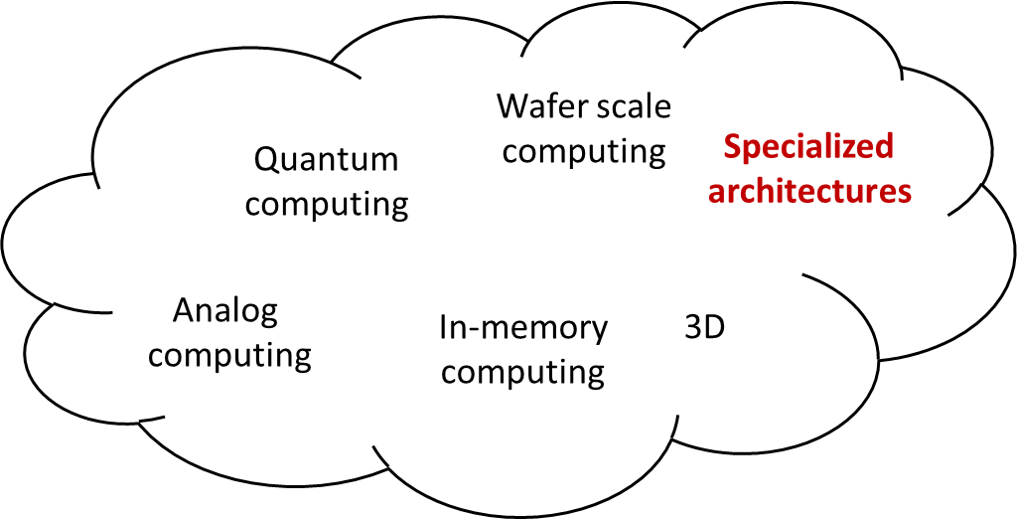
\includegraphics[width=0.7\linewidth]{figures/cloud.png}
% \caption{Innovative approaches for acceleration of CNN workloads}
% \label{fig:cloud}
% \end{figure}

% \subsubsection{Conventional CMOS hardware}

Less risky approaches focus on moving away from traditional von Neumann architectures, using specialization of compute architectures to provide the necessary performance scaling and energy efficiency. 
Due to the specialization, the devices become increasingly heterogeneous.
A huge range of devices has emerged that all try to address this problem in different ways, whereby the key challenge is:
How do we loop transform and unfold the algorithms best to maximize data reuse and compute efficiency, minimize memory bottlenecks, and limit power consumption while meeting real-time requirements? 
In the following, we restrict our discussion to the devices that can be realistically used today, and thereby focus on \textbf{specialized architectures}. 
\textcolor{red}{[S.H. This statement seems out of place.  What is "speculative approaches" referring to?]It is important to remember though that these speculative approaches, as discussed above, will materialize in the future and we will have to deal with an even greater diversity of hardware platforms.}

The choice of hardware type and quantity often boils down to a set of constraints imposed by compute environment (datacenter, cloud, on-premise, edge, mobile), workload type (inference, training), data type (Language, Time Series, Vision, Graph, etc), ML model, usage model (online inference, batch jobs), and user-centric Service-Level Agreements (encryption level, request latency, etc). For large datacenter deployments handling various types of workloads, it is often the case that several platforms must be combined to reduce Total Cost of Ownership (ToC) across all their hardware platforms. It has therefore become increasingly necessary for owners of heterogeneous platforms to think of their systems as large-scale multi-processor computers, a trend sometimes termed Warehouse Scale Computing~\cite{wsc}. For Deep Learning hardware accelerators, these new computers generally take the form of CPU co-processors: a host CPU communicates with other entities in the datacenter, interfaces with disk memory, and formats input data which is then offloaded to the accelerator responsible for executing a user-defined compute graph, or Neural Network. 

We begin with a taxonomy of these hardware architectures, and discuss their relevant characteristics when it comes to acceleration of machine learning workloads. 
This is essential to understand how they will differ in their execution behavior, what it takes to leverage their unique features and how they can potentially benefit from previously introduced optimization techniques. 
% We will also discuss deployment options that are unique to specific architectures, and may or may not bring additional benefits to CNN inference. 
% At last, we briefly touch on other considerations such as form factors. All of these stipulate another form of design requirements for a benchmarking methodology.

%%%%%%%%%%%%%%%%%%%%%%%%%%%%%%%%%%%%%%%%%%%%%%%%%%%%%%%%%%%%
\subsubsection*{\textbf{Taxonomy of Compute Architectures for Deep Learning}}

\begin{figure*}
\centering
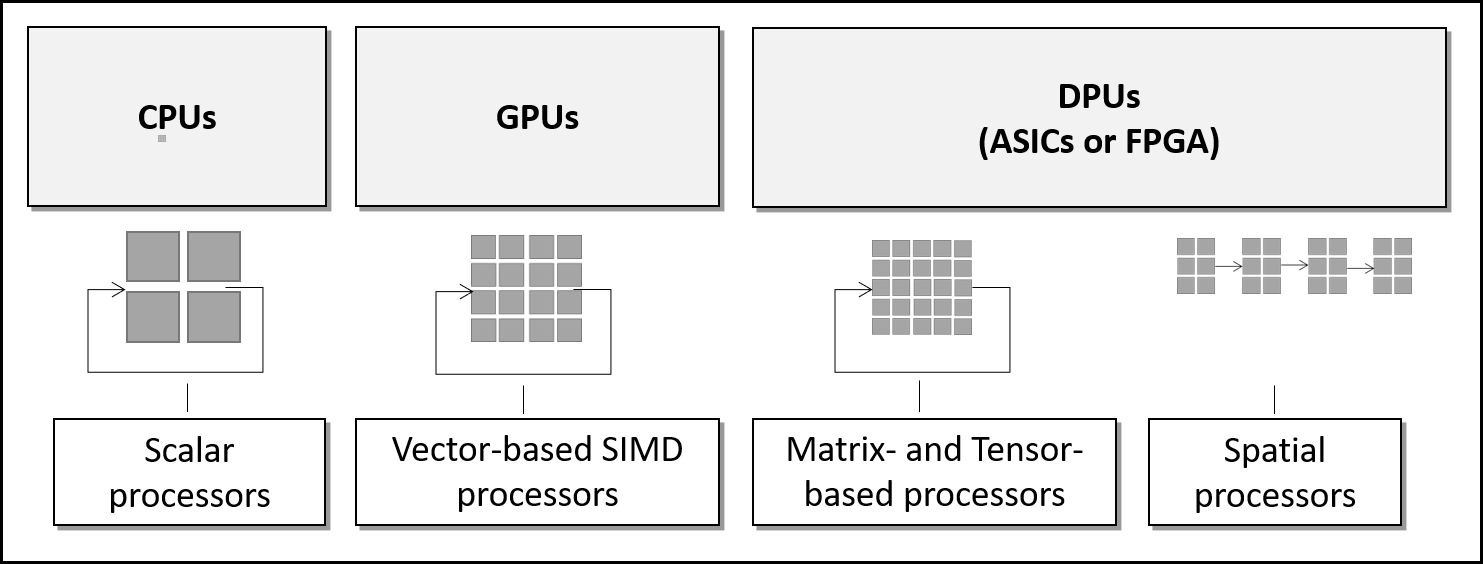
\includegraphics[width=0.8\linewidth]{figures/taxonomy.png}
\caption{Taxonomy of compute architectures, differentiating CPUs, GPUs and DPUs}
\label{fig:tax}
\end{figure*}

A broad range of hardware architectures to deploy machine learning algorithms exists today.
We can broadly classify them by the following criteria:

\begin{enumerate}[itemsep=-1pt]
\item Basic type of compute operation
\item Inherent support for specific numerical representations
\item External memory capacity (which is mostly relevant for training workloads)~\footnote{In these comparisons, we treat HBM and HBM2 as external memory as it is used in the same way as DDR4 or GDDR memory.}
\item External memory access bandwidth
\item Power consumption in the form of thermal design power (TDP)
\item Level of parallelism in the architecture and the degree of specialization
\end{enumerate}
 
As is shown in Figure~\ref{fig:tax}, we classify the compute architectures into scalar processors (\textbf{CPUs}), vector-based processors (\textbf{GPUs}), and so-called deep learning processing units (\textbf{DPUs}), although realistically these categories blend to some degree. 
DPUs are specialized for this application domain whereby we distinguish the more generic matrix- or tensor-based processor and a spatial processing approach. DPUs can be implemented with either ASICs or FPGAs. All of these architectures will be discussed individually below.

\paragraph*{CPUs} CPUs are widely used for ML applications, and are viewed as largely serial or scalar compute engines (even though high-end variants for cloud deployment may have up to 10s of cores). They are optimized for single thread performance, with implicitly managed memory hierarchies (with multiple levels of caches), and support floating point operations (FP64 and FP32) as well as 8bit and 16bit integer formats with dedicated vector units in most recent variants. Theoretical peak performance tops at 6.8TOPs for FP64 assuming boost clock speed (Cascade lake, 56 cores, 3.8GHz). External memory is currently primarily leveraging DDR4 memory banks with large capacities: Intel's Cascade Lake offers up to 4.5 TebiByte ($2^{40}$ Bytes) which is beyond what any of the other device categories can offer. Access is at maximum speed through high-end hardened memory controllers, offering 282~Gbps bandwidth (for example Cascade Lake with 12 DDR4 channels). 
\textcolor{red}{[S.H. This sentence is confusing and should be rewritten]In regards to memory bandwidth, this is overall at the lower end of the spectrum, however in many application contexts, this can be compensated through the sophisticated multi-level memory hierarchies.}
Regarding power consumption, CPUs are at the upper end of the spectrum with high-end devices range up to 400\,W~\cite{cascadelake}.
In the embedded space, ARM processors provide generally popular solutions, in particular when performance requirements are very low and when functionality is required that is not supported by the specialized device variants. In particular, the \textcolor{red}{[S.H. Missing reference]Ethos~\cite{} }family of processing cores is specialized for CNN workloads and as such is considered under the DPU category below.
Advantages of CPUs are the generality of the hardware, as well as the ease of programming where design environments have matured over decades. 
As expected this comes at the cost of lower peak performance and less efficiency compared to the more specialized device families.
In regards to quantization, CPUs can only leverage this optimization technique for INT8 and INT16 if supported.

\paragraph*{GPUs} GPUs are SIMD-based (Single Instruction, Multiple Data) vector processors that support smaller floating point formats (FP16) natively, as well as fixed point 8-bit and 4-bit integer formats more recently, and have a mix of implicitly and explicitly managed memory. 
NVIDIA GPUs are some of the most popular hardware targets for machine learning, and newer families of chips have been introduced to specifically accelerate this workload, with AMD not far behind. 
The latest devices in NVIDIA's Volta and Turing architecture families, introduced in 2018 and 2019 respectively, offer up 130TOPs in FP16, which is beyond the capabilities of the latest CPU generations. 
As such they are amongst the highest performant devices in the market for the acceleration of DNNs as they can exploit the high degree of parallelism inherent in this application via increasingly specialized architectural features.
For example, NVIDIA's Volta is the first generation to incorporate tensor cores as a new feature, as well as improved FP32 and FP64 support for training in a data center setting~\cite{NVIDIAv100}, and also introduced a deep learning accelerator (DLA) in their embedded devices to further reduce power consumption. This specialization brings additional challenges for their usage; there are up to 3 distinct execution units now, namely CUDA cores, tensor cores and the DLA, which don't operate on the workload simultaneously (at least not easily or by default). 
We therefore don't sum up the peak performance of different execution units, but use only the maximum.
AMD announced the Vega GPU~\cite{RadeonInstinctGPU} with new deep learning instruction set operations, with the goal of obtaining parity with NVIDIA's high-end Tesla V100 datacenter GPUs.  Also, AMD's  most recent EPYC family supports customized instructions for deep learning~\cite{epyc}. 
Both companies offer also low power GPUs for the embedded space, namely the AMD Vega mobile GPU~\cite{radeon-mobile} and NVIDIA Jetson TX2~\cite{nvidia-jetson} and AGX family~\cite{agx}.

In regards to memory, GPUs leverage specialized and highly pipelined GDDR memory, which reduces capacity, but offers much higher bandwidth (up to 732GBps). With NVIDIA's Turing family the latest devices include HBM2 DDR memory stacks~\cite{turing}, which scales the memory access bandwidth to 1TBps and beyond. 
Again this is particularly important to address the needs of training workloads.
For the same reason some of the DPUs introduce HBM2 as well, as discussed below. 
In regards to power consumption, GPUs are high, up to 345\,W.

One general challenge for GPUs is that they need to leverage input parallelism to achieve high utilization of their large compute arrays. Therefore before execution inputs need to be grouped into batches, which has adverse affects on end latency. 
% This is discussed in more detail below in Section~\ref{sec:deploy}. 
Further, GPUs are relatively high in power consumption.
Regarding quantization, support is limited to the inherent datatypes, which are INT4 at smallest in the context of NVIDIA's Turing family, and INT8 for many of the others.
Finally, the corresponding software environments for GPUs, while not on the same level as CPUs, have matured significantly and provide increasing ease of use.

\paragraph*{FPGAs and ASICs}
FPGA and ASIC customize hardware architectures to the specifics of a given application.
They can be adapted in all aspects to suit a use case's specific requirements.
This includes their IO capability, their functionality, or even to suit specific performance or efficiency targets. 
FPGAs can be reprogrammed whereas ASICs are fully hardened.
This flexibility allows for amortizing the design costs of the circuit across many applications, but comes at the expense of hardware resource cost and performance.

FPGAs are a popular choice for acceleration of CNNs. 
Traditionally, an FPGA compute fabric consist of a sea of lookup tables (LUTs) which are interconnected through a programmable interconnect. The latest generations host millions of LUTs. Furthermore, the fabric is interspersed with specialized hardened compute blocks (DSPs) which accelerate n-bit multiply accumulate operations (MACs), as well as SRAM blocks. The latter are referred to as block RAMs (BRAMs), which hold 36~kbits, and Ultra RAMs (URAMs) which store 288~kbits.
More recent FPGA generations combine multiple FPGA dies, referred to as super logic regions (SLRs), and leverage a silicon interposer to provide connectivity between SLRs. 
This technology is referred to as stacked silicon interconnect (SSIT) and helps scale device capacity.

\paragraph*{DPUs} As mentioned at the beginning, the term DPU (short for deep learning processing unit) refers to a new type of compute architecture, specialized for the acceleration of CNNs. 
DPUs are customized for these type of applications in a number of ways: types of operations supported, direct support of tensors or matrices, inherent data types and supported numerical representations, macro-architecture, explicitly managed and specialized memory hierarchies, and which levels of parallelism they exploit (input, output pixel, IFM, OFM, bit, and layer and branch parallelism) as was introduced in the first part of this chapter.
We differentiate two types of DPUs, which can be implemented with both ASIC technology and FPGAs.

\begin{figure*}[h!]
\centering
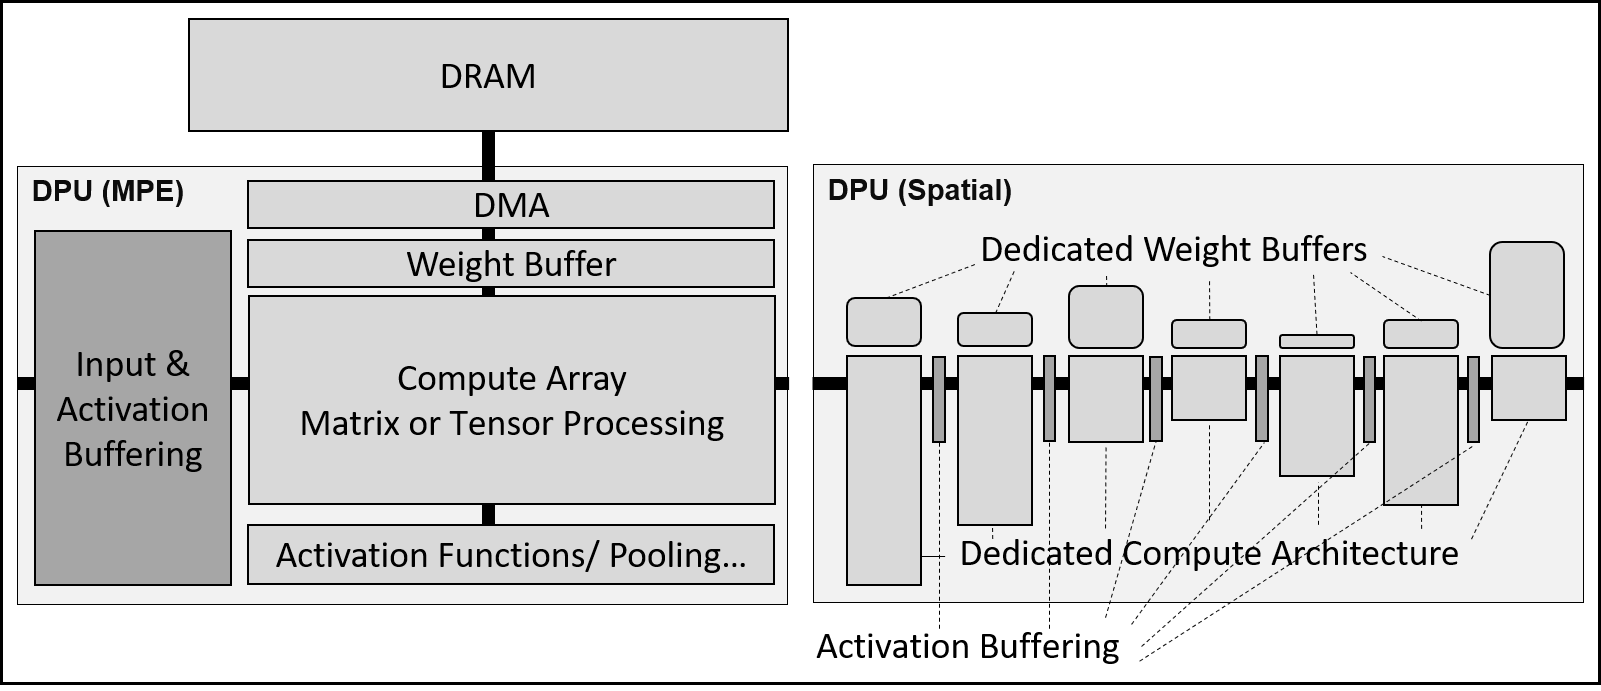
\includegraphics[width=0.8\linewidth]{figures/dpu1.png}
\caption{DPU architectures: Matrix of Processing Engines (MPE) on the left, and spatial architecture on the right}
\label{fig:dpu}
\end{figure*}

\paragraph*{Matrix of Processing Elements (MPE)} The first type, as shown in the left side of Figure~\ref{fig:dpu}, consists of a MPE that operates on matrices or higher dimensional tensors. The processing engines can be simple MACs, vector processors, or more complex VLIW (Very Long Instruction Word) cores which can support concurrent execution of different instructions.
A popular example in this category is Google's Tensor Processing Unit (TPU).  
Introduced in 2016~\cite{tpu1}, it was originally designed to accelerate Google's TensorFlow framework.
The first generation supported integer arithmetic with a massively parallel INT8 matrix-multiply engine.
The second generation TPU was announced in May 2017~\cite{tpu}, and the third generation in May 2018~\cite{tpu3}.
These newer chips boast improved memory performance as well as support for floating point specifically aimed at training.  
There are a number of startups introducing custom hardware which fall into this category.
Within the cloud space there are Graphcore, Groq, and Wave Computing.
Within the embedded space, where the design constraints are even more stringent, we find even more solutions. %, as are listed in Table~\ref{tableHW-embedded}.
Most are secretive about the details of their designs. Intel is investigating several custom accelerators and has for that purpose acquired a number of startups, namely Nervana, Habana and Movidius. Fathom~\cite{movidius-tom} is Movidius' ultra low power Neural Compute Stick (NCS) which operates at about 1\,W.  
Also, ARM offers specialized CNN processors in the form of their Ethos family, boosting performance up to 4TOPs with support for INT8 and INT16 datatypes.

\textcolor{red}{[S.H. Edits needed to the DPU architectures figure: (1) move the left and right further apart - hard to see the separation.  Remove the black box around everything.  Adjust spacing on / between Functions and Pooling.  Remove ... from Pooling]}

As mentioned above, DPUs provide specialized datatypes to execute heavily quantized, reduced precision CNN implementations.
At the extreme, binarized neural networks (which are very high throughput at extremely low power) are exploited in the following ASICs: BinarEye~\cite{binareye}, BNN Custom Fabric~\cite{ando2017brein}, and IBM AI Accelerator~\cite{IBMAI}. Also, Lattice has announced binarized neural network libraries targeting low power FPGA and achieving 1\,TOPs/W~\cite{lattice-bnn}.
Custom floating point representations are also considered. For example, Microsoft's Brainwave project~\cite{chung2018serving} uses this approach with the aim at applying FPGAs to CNNs at datacenter scale.
However, typically the hardened versions in ASICs only support INT8, as lower precisions could potentially limit their application scope. FPGA-based MPE implementations such as Xilinx's xDNN are less constrained and in principle can be customized as needed.

Similar to the GPU, but perhaps to a lesser degree, DPUs leverage input, IFM (input feature map) and OFM (output feature map) parallelism, which requires buffering of inputs and may have adverse affects on latency as well.
A particular challenge arises in the context of software environments, which differ for all vendors and are less mature than what we have observed for CPUs and GPUs. Typically, they are limited to support execution of very specific layer types (sometimes even restricted in regards to parameter ranges) and neural networks. \textcolor{red}{[S.H. This statement is a bit awkward.  Please rewrite]A given and increasingly expanding modelzoo is supported, however many limitations exist in the form of layer types and are provided as black box solutions which lack transparency and flexibility.} 

In summary, through their specialization these implementations minimize hardware cost, maximize performance and optimize efficiency by exploiting specific precision arithmetic with a specialized instruction set and customized memory system. However, in order to gain the performance advantage the algorithms need to be adapted to leverage these features. 

\paragraph*{Spatial DPUs.} The second type of DPU leverages spatial acceleration and exploits layer and branch parallelism. Popular examples are hls4ml~\cite{hls4mldata_150p} and FINN~\cite{umuroglu2017finn,blott2018finnr}.
To that extent, the hardware architecture is even further specialized to the specifics of a given deep learning topology. 
This is visualized in the right side of Figure~\ref{fig:dpu}. 
The hardware architecture actually mimics the given deep learning topology and the inputs are streamed through the architecture. 
Every layer is instantiated with a dedicated compute datapath. 
Each layer has a dedicated weight buffer, and activation buffers in-between layers are FIFOs of minimal size. They buffer just enough data to feed the next set of convolutions in the next layer. 
This is substantially more efficient compared to the first type of DPUs or GPUs and yields reduced latency. 
%, where all activations between 2 layers for a full batch of images need to be double-buffered. 

DPUs and GPUs generally perform a layer by layer compute, where a sequence of images has to be buffered in order to extract maximum compute out of the platform (input, IFM and OFM parallelism). 
For this the device buffers a batch of images before computing the first layer of all images. 
Then all intermediate results are buffered, and then the next layer is computed and so on. Hence the latency is heavily dependent on the size of the input batch.

As a result, spatial DPUs have an advantage in regards to latency.
This level of customization is only possible with programmable hardware architectures such as FPGAs, as they can adapt the hardware architecture for different use cases. 
This generally wouldn't make sense in the context of an ASIC accelerator, as that would yield an ASIC only capable of accelerating one specific topology, which would be far too restrictive in scope.
The limitation in spatial architectures is the scalability in numbers of layers. 
Each layer comes at a resource cost overhead and there is a maximum number of layers that can be created within a single device. As a result some extremely deep CNNs might not be able to fit into a single device. Microsoft's Brainwave project leverages spatial computing and overcomes this limitation with a distributed approach~\cite{chung2018serving}.

Once a spatial DPU has been leveraged and the architecture is specialized for a very specific CNN, the architecture can be further customized in regards to minimum precision.  By supporting only the bits as needed per layer of the CNN they can achieve even higher performance and efficiency, while in an MPE, the hardware will support the maximum precision that is required over the whole network. In regards to customized precisions and spatial architectures, FINN has pioneered the first binarized neural network accelerators \cite{umuroglu2017finn,fraser2017scaling} and provided many proof points for customized reduced precision implementations~\cite{blott2018finnr}. 
This flexibility comes at a cost, in the form of programming complexity, and they are extremely difficult to characterize in general, as the performance characteristics depend on the specifics of the hardware architecture that has been implemented.

\paragraph*{Further Variants}
\textcolor{red}{[S.H. This section is kinda abrupt.  Cut, or smooth the transitions into it.  Also, how does the next paragraph relate to this section?]
Others exploit sparse computing engines, such as EIE and its successor ESE~\cite{han2017ese}, SCNN~\cite{parashar2017scnn}, Cnvlutin~\cite{cnvlutin}, Cambricon-S and Cambricon-X~\cite{zhang2016cambricon}. These are the only architectures which can benefit from irregular sparsity.}

% \begin{figure}[h!]
% \centering
% 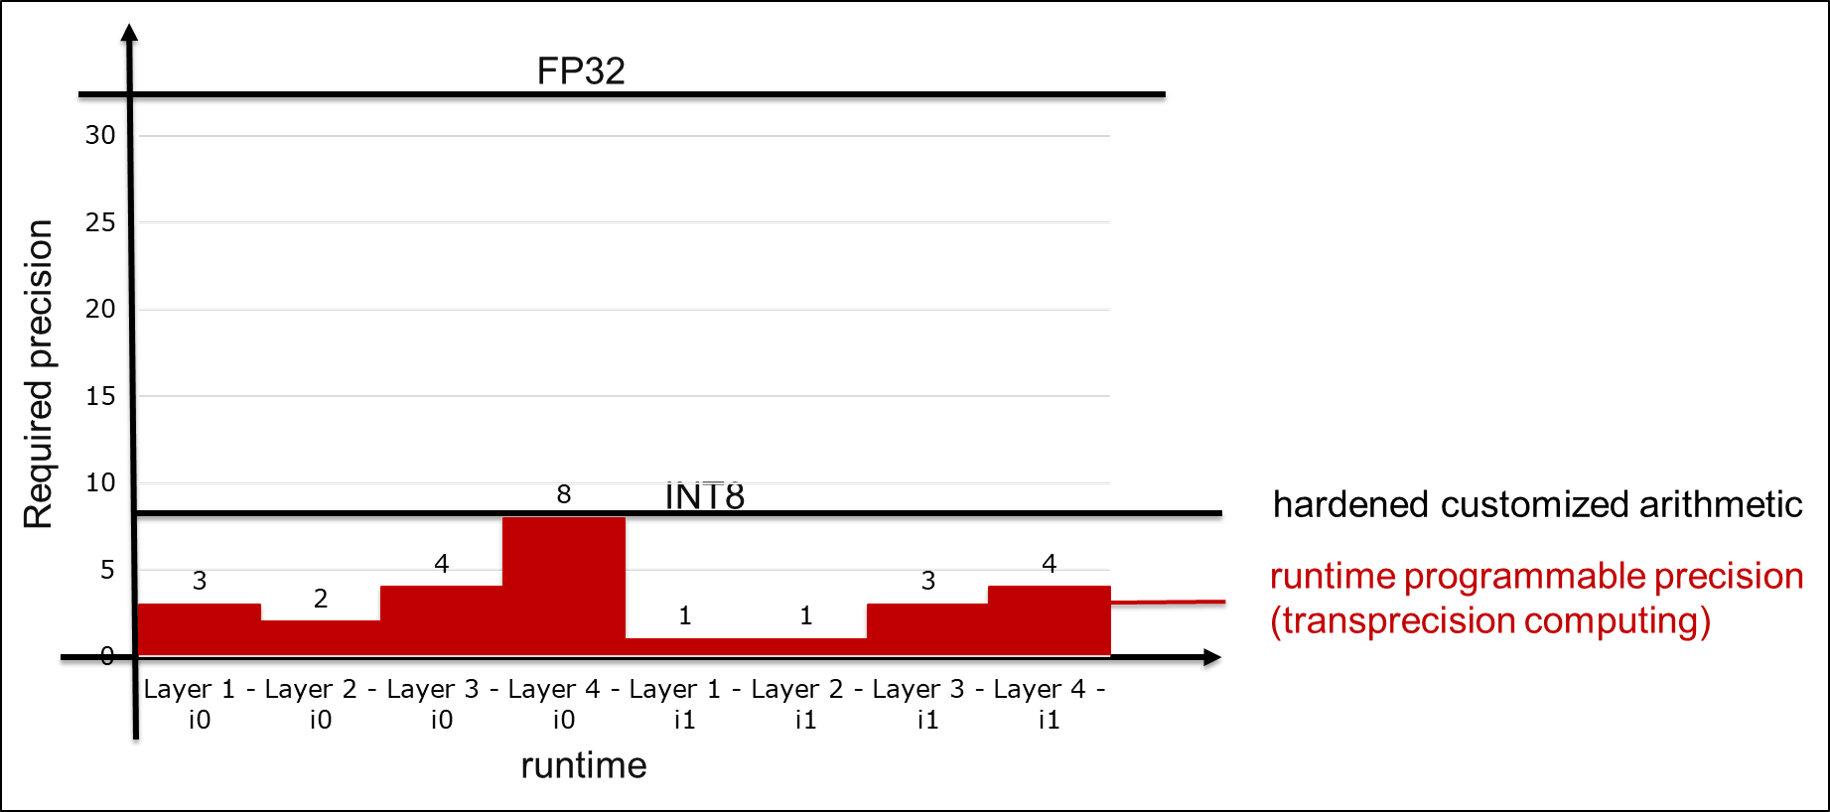
\includegraphics[width=0.6\linewidth]{figures/runtime_preicison.png}
% \caption{Run-time programmable precision.}
% \label{fig:bismo}
% \end{figure}

Finally, another dimension for customization of precision is to optimize over the execution- or run-time of a CNN.
In other words, beyond using statically fixed reduced precision, where the hardware operates with a fixed precision for all variables, some approaches explore run-time configurable bit precision which allows for the exploitation of bit-parallelism in the arithmetic. 
% This is also referred to as transprecision computing and illustrated in Figure~\ref{fig:bismo}. 
% On the x-axis, we show the execution time of a CNN, where we first execute all layers (layer 1, layer 2 and so on) for input i0.
% Then we progress to the second input i1 and so on.
% The y-axis annotates the minimum precision required.
% In the shown example, layer 1 for i0 requires 3bits, while layer 2 for i0 requires 2bits.
% This can vary for every input.
% In case of a FP32 implementation, marked by the top line, the area between the red boxes and line would be representative of the wasted computation.
% When leveraging hardened customized arithmetic, for example INT8, then the wasted computation is significantly reduced, but there is further scope for optimization.
On the hardware implementation side, this can be exploited with run-time programmable precision and is effective with \textbf{bit-serial} implementations. 
For example Umuroglu et al.~\cite{umuroglu2018BISMO} demonstrate with BISMO that bit-serial can provide highly attractive performance with minimal overhead on FPGAs, while Judd et al. show the same is true for ASICs with their prototype ASIC called Stripes~\cite{judd2016stripes}. 
While this concept can be applied to both MPE and spatial architectures, it makes most sense for MPEs.

% \subsubsection{Example Platforms for Cloud and Embedded Systems}
% We have carried out extensive research on available hardware platforms in this space and collected and summarized them in Tables~\ref{tableHW-cloud} and \ref{tableHW-embedded} with published performance and power. 
% These tables cover both high-end platforms for cloud deployment as well as devices targeted for IoT.

% {\small
% \begin{table}
% \caption{Hardware architectures for cloud systems with theoretical performance}
% \label{tableHW-cloud}
% \begin{center}
% \resizebox{\textwidth}{!}{
% \begin{tabular}{|l|ccccc|}
% \toprule
% \textbf{Platform}&\textbf{Num. Choice}& \textbf{Throughput [TOPs]}&\textbf{Mem BW [GBps]} & \textbf{Power [W]}&\textbf{Performance/Power [TOPs/W]}\\\midrule
%  \textbf{CPUs} & & & & & \\ \hline
% Intel CascadeLake 92xx (56cores) ~\cite{cascadelake} & FP64 & 6.8 & 282 & 400 & 0.017 \\
% Intel CascadeLake 82xx (28cores) ~\cite{cascadelake} & FP64 & 3.5 & 141 & 205 & 0.017 \\
% AMD Epyc 7742 (28cores) ~\cite{epyc} & FP64 & 3.5 & 205 & 225 & 0.016 \\\midrule
%  \textbf{GPUs} & & & & & \\ \hline
% Quadro RTX 6000~\cite{turing} & FP16 & 130.5$^\star$ & 624 & 260 & 0.5 \\
% NVIDIA V100~\cite{NVIDIAv100} & FP32 & 14 & 250 & 300 & 0.06 \\
% NVIDIA V100 & FP16 & 112$^\star$  & 250 & 300 & 0.45 \\
% %NVIDIA P100~\cite{NVIDIAp100} & FP32 &   8 & 732 & & \\
% %NVIDIA P100 & FP16 & 16 & 732  & & \\
% %NVIDIA P40~\cite{NVIDIAp40} & INT8 & 47 & 200 & 346 & 0.24 \\
% %NVIDIA P4  & INT8 & 22 & 60 & 192 & 0.37 \\
% AMD Vega10~\cite{AMDVega} & FP32 & 13.7 & 484 & 345 & 0.04\\\midrule
%  \textbf{TPUs} & & & & & \\ 
% Google TPUv1~\cite{tpu1} & INT8 & 92 & 75 & 34 & 1.23 \\
% Google TPUv2~\cite{tpu} & FP16 & 45 &  & 600 &  \\
% Google TPUv3~\cite{tpu3} & FP16 & 90 &  &  &  \\\midrule
%  \textbf{ASIC DPU (MPE)} & & & & & \\ \hline
% Graphcore & Custom & 224 & & 300 & 0.75 \\
% Groq & unknown & 400 & & & 8 \\
% Nervana & custom16 & 55 & & & \\
% Wavecomputing 1DPU & INT8 & 181 & & 271 & 0.7 \\\midrule
%  \textbf{FPGA-based Spatial DPU} & & & & & \\ \hline
% Xilinx VU9P	&2b/8b	&93.00	&88	&100	&1.06\\
% Xilinx VU9P	&2b/4b	&139.88	&88	&100	&1.59\\
% Xilinx VU9P	&2b/2b	&192.52	&88	&100	&2.19\\
% Microsoft Brainwave Stratix X~\cite{chung2018serving} & FP8 & 90 & & 125 & 0.72  \\
% \midrule
% \multicolumn{6}{l}{Performance of Tensor Cores $^\star$} \\
% \end{tabular}
% } 
% \end{center}
% \end{table}}

% {\small
% \begin{table}
% \caption{Low power hardware architectures and theoretical performance}
% \label{tableHW-embedded}
% \begin{center}
% \resizebox{\textwidth}{!}{
% \begin{tabular}{|l|ccccc|}
% \toprule
% \textbf{Platform}&\textbf{Num. Choice}& \textbf{Throughput [TOPs]}&\textbf{Mem BW [GBps]} & \textbf{Power [W]}&\textbf{Performance/Power [TOPs/W]}\\\midrule
% \textbf{CPUs} & & & & & \\ \hline
% ARM Cortex-A53 using gemmlowp; Ultra96 & INT8 & 0.192 & 4.26 &  &  \\
% Bitserial Cortex-A57; Jetson TX1~\cite{umuroglu2017streamlined} & BIN & 0.09 &  &  & 0.019 \\\midrule
%  \textbf{GPUs} & & & & & \\ \hline
% NVIDIA AGX (30W)~\cite{agx} & FP32 & 3.59 & & 30W & 0.12 \\ 
% NVIDIA AGX (30W)~\cite{agx} & FP16 & 7.19 & & 30W & 0.24 \\ 
% NVIDIA TX2 (MaxP)~\cite{nvidia-jetson} & FP32 & .575 & 59.7 & 15.0 & 0.038\\
% NVIDIA TX2 (MaxP)~\cite{nvidia-jetson} & FP16 & 1.15 & 59.7 & 15.0 & 0.077\\\midrule
%  \textbf{ASIC DPU} & & & & & \\ \hline
% Movidius Myriad 2~\cite{movidius-tom} &  INT8 & .15  &  & 1.2 & 0.125 \\
% Movidius Myriad X~\cite{myriadx1} &  INT8 &  1 &  & 1 & 1 \\
% Kalray MPPA Turbocard3~\cite{kalray} & FP32 & 1.6 &  & 110 & 0.014 \\
% BinarEye~\cite{binareye} & BIN & 0.09 - 2.8$^\star$ & & & 230$^\dagger$\\
% BNN Custom Fabric~\cite{ando2017brein} & BIN & 1.4 & & 0.6 & 2.3\\
% Stripes Bitserial ASIC~\cite{judd2016stripes} & BIN & 128.5 & & & 4.3\\
% IBM AI Accelerator~\cite{IBMAI}\footnote{We will add the VLSI reference as soon as it becomes live} & BIN & 12 & & & \\
% Eyeriss~\cite{chen2017eyeriss} & INT16 & 0.084 & & 1.17 & $^\dagger$\\
% ARM ML Processor~\cite{trillium} & unknown & 4.6 &  &  & 3 \\
% DianNao~\cite{chen2016diannao} & INT16 & 0.452 & 120 & 0.485 & 0.93\\
% EIE(28nm)~\cite{han2016eie} & INT4 & 3 (0.102 sparse) & 2.36 & 1.27 & 2.4 (0.08 sparse)\\
% Cambricon-X~\cite{zhang2016cambricon}  & INT16 & 0.544 &  &  & \\
% \midrule
%  \textbf{FPGA DPU} & & & & & \\ \hline
% Lattice SenseAI~\cite{lattice-bnn}  & BIN & 1.4 & & 0.6 & 2.3\\
% BISMO biserial on PYNQ~\cite{umuroglu2018BISMO}& BIN & 6.5 &  & 4.64 & 1.4 \\
% FINN on ZC706~\cite{umuroglu2017finn} & BIN & 11.6 & & & 0.408 \\
% ZCU104 (Deephi-666MHz)      & INT8 & 4.60 & 19.2 & %12 
% & \\ %0.38 \\
% ZCU104 (Theoretical-775MHz) & INT8 & 5.36 & 19.2 & %12 
% & \\ %0.45 \\
% GX1150 on HARPv2~\cite{moss2018customizable} & BIN & 0.041 & & & 0.85 \\
% \midrule
% \multicolumn{6}{l}{Measured $^\star$} \\
% \multicolumn{6}{l}{Chip level power consumption only $^\dagger$} \\
% \end{tabular}
% } 
% \end{center}
% \end{table}}

% \paragraph*{Comparison}
% Roughly comparing these architectures, we can distinguish between them in regards to their theoretical peak throughput, latency, power consumption, external memory capacity and memory access bandwidth, their degree of specialization of the hardware towards the workload and the associated ease of use.
% CPUs count as general purpose devices, even though they also show first signs of specialization in regards to CNN acceleration with specialized instructions in their vector processing units. For example Intel's AVX-512 now offers so-called Vector Neural Network Instructions (VNNI)~\cite{avx512}. However, overall they show the least degree of specialization. CPUs provide high throughput, are the highest in regards to power consumption and memory capacity and the easiest to use.
% GPUs increasingly specialize for AI workloads and support increasingly reduced precision types (INT4 with the latest Turing family of GPUs) and specialized tensor processing cores. They offer together with DPUs highest performance and excel at external memory bandwidth but also at a high power footprint and very high latency cost. 
% DPUs, due to their increasing degree of specialization, offer top in class in regards to throughput, energy efficiency and with spatial DPUs offering lowest latency. However, increasing hardware complexity is accompanied with increasing complexity in the design entry, which reduces ease of use.
% We have illustrated these characteristics in Figure~\ref{fig:hwradarheat}. On the left side, the heatmap visualizes through colour the qualitative characteristics and highlights the strong aspects of each architecture. The number reflects a ranking, whereby higher is better. Similarly, the radar chart depicts the compromises in each approach and illustrates that there is not a single architecture that excels in all aspects.

% \begin{figure}[h!]
% \centering
% 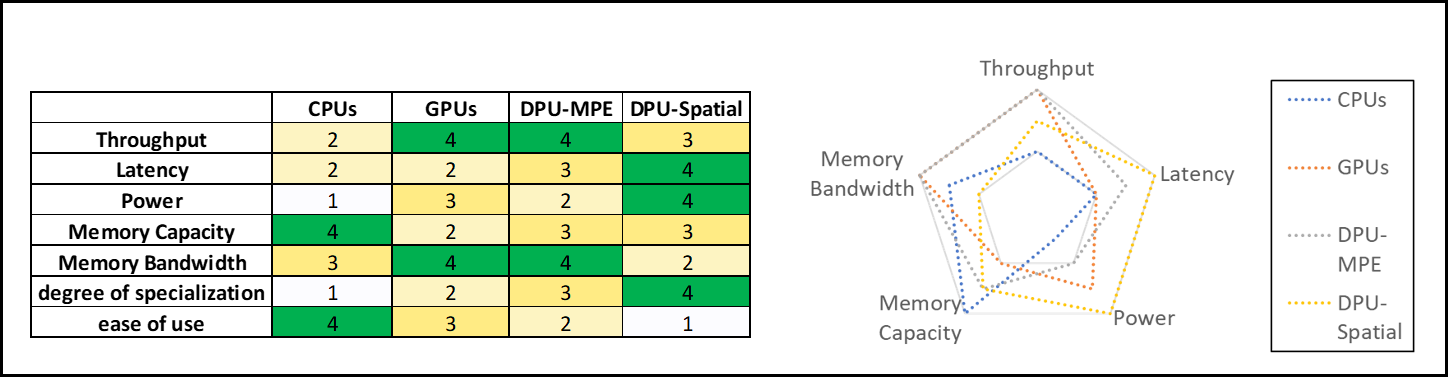
\includegraphics[width=1.0\linewidth]{figures/hwradarheat.png}
% \caption{Qualitative comparison of hardware architectures}
% \label{fig:hwradarheat}
% \end{figure}

% \paragraph*{Trends.}
% As already indicated, with newer generations, the boundaries between different hardware architectures are blurring. CPUs are increasingly incorporating vector processing units and support for reduced precision integer formats. GPUs are adding tensor processing units, and the TPU now supports floating point operations.
% FPGAs can support any of the above configurations with explicitly managed memory. They are the most flexible of all target hardware, and can be configured to support any numeric representation.

% %%%%%%%%%%%%%%%%%%%%%%%%%%%%%%%%%%%%%%%%%%%%%%%%%%%%%%%%%%%%%%%%%%%%%%%%%%%%%%
% \subsubsection{Deployment Options}
% \label{sec:deploy}

% Many of the described hardware platforms offer different deployment options in order to support different compromises between throughput, latency and power as indicated in Figure~\ref{fig:powermodes}. These are discussed in more detail within this section. In our benchmark, we ensure to cover a systematic exploration of all of the provided deployment options regarding all figures of merit to ensure a fair comparison and thorough understanding of the design compromises.
% \begin{figure}[h!]
% \centering
% 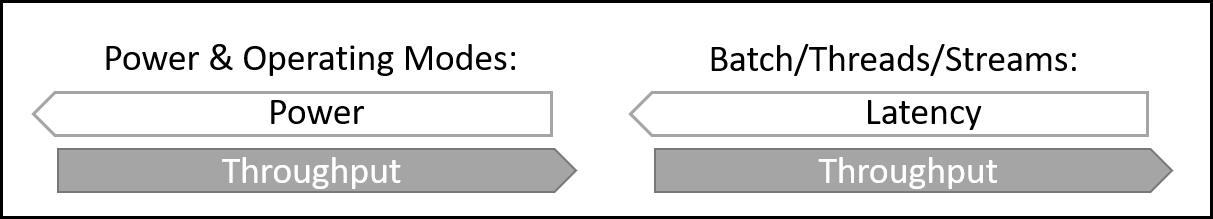
\includegraphics[width=0.9\linewidth]{figures/powermode.png}
% \caption{Compromises between power, throughput and latency with deployment options}
% \label{fig:powermodes}
% \end{figure} 

% \paragraph*{Operating and Power Modes.}
% Many of the chosen platforms offer different power or operating modes which provide a compromise between power consumption and achievable throughput, for example by regulating clock speed or disabling parts of the circuit. A specific example, is the TPU Coral stick from Google which can operate with a fast or a slow clock. The NVIDIA GPU Jetson TX2 platform can run in either maxn, maxp or maxq modes. Maxn is the high performance mode with highest power consumption. Maxp is the most efficient mode, with lowest power but also lowest performance, and maxq is a compromise between maxn and maxp. 
% Similarly, the NVIDIA AGX offers a maxn, 10W, 15W or 30W mode. 
% Examples of this behaviour are shown in Figure~\ref{fig:pwrperf} indicating substantial differences in regards to power and performance for different modes, where naturally higher performance comes with higher power consumption.
% \begin{figure}[h!]
% \centering
% 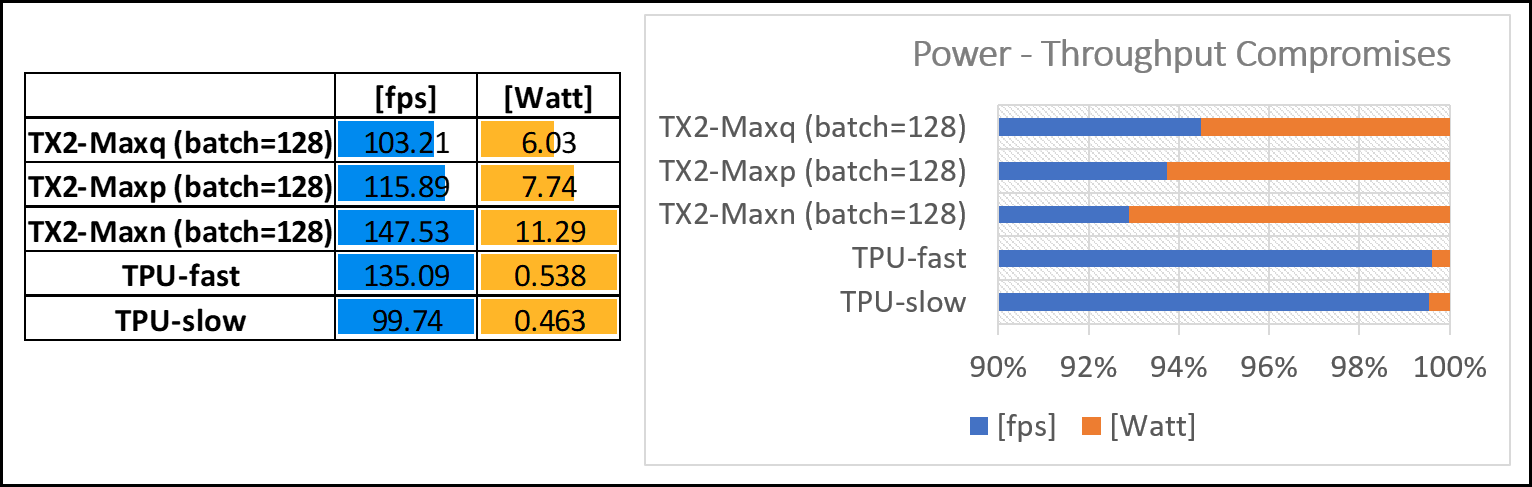
\includegraphics[width=0.9\linewidth]{figures/pwrvsperf.png}
% \caption{Power versus performance for GoogLeNetv1: Different trade-offs are achieved in different operating modes}
% \label{fig:pwrperf}
% \end{figure} 

% \paragraph*{Batch Sizes, Thread Counts and Stream Sizes.}
% Many hardware platforms require increased batch sizes, thread counts or stream sizes in order to extract maximum performance out of a hardware platform and achieve high compute efficiency. However, this can result in substantially different latency as is shown in Figure~\ref{fig:latfps1}. 
% Layer-by-layer compute architectures including Google's TPU, GPUs such as Nvivida's TX2, and Intel's Neural Compute Stick {NCS)} have a larger than linear increase in latency with regards to batch size. 
% Typically, a sequence of images has to be buffered in order to extract maximum compute out of the platform. 
% The architecture buffers a batch of images before computing the first layer of all images. Then all intermediate results are buffered, and then the next layer is computed and so on. 
% Hence the latency is heavily dependent on the batch size (or thread count). 
% As the device utilization saturates with increasing batch size, peak performance is reached, and no further benefit can be achieved. 
% This is illustrated by the measured results for the NCS and TX2.

% Spatial architectures such as the dataflow implementations with FINN~\cite{umuroglu2017finn} have a fixed latency independent of input stream size which is determined by the length of the given pipeline and is fixed.
% This is visualized with the gray line in the Figure which represents the measurements on a spatial architecture.
% As such when only 1 input is processed (stream size=1) the pipeline is underutilized and throughput is low.
% Full throughput is achieved when the stream size saturates the pipeline, whereby the latency remains constant independent of the stream size.
% Finally, the Xilinx DPU example (implemented on a ZCU102 development platform), which deploys a vector of processing engine, utlizes thread counts rather than batches.
% Latency increases with rising thread count, however at a much gentler slope than batch sizes for GPUs. 
% Example behaviour of latency and performance for a spectrum of batch sizes, thread counts and stream sizes is shown in Figure~\ref{fig:latfps1} for the above mentioned devices for ResNet50v1 implementations (RN50) and a VGG16 derivative CNN, currently abbreviated as CNV100\%.

% \begin{figure}[h!]
% \centering
% 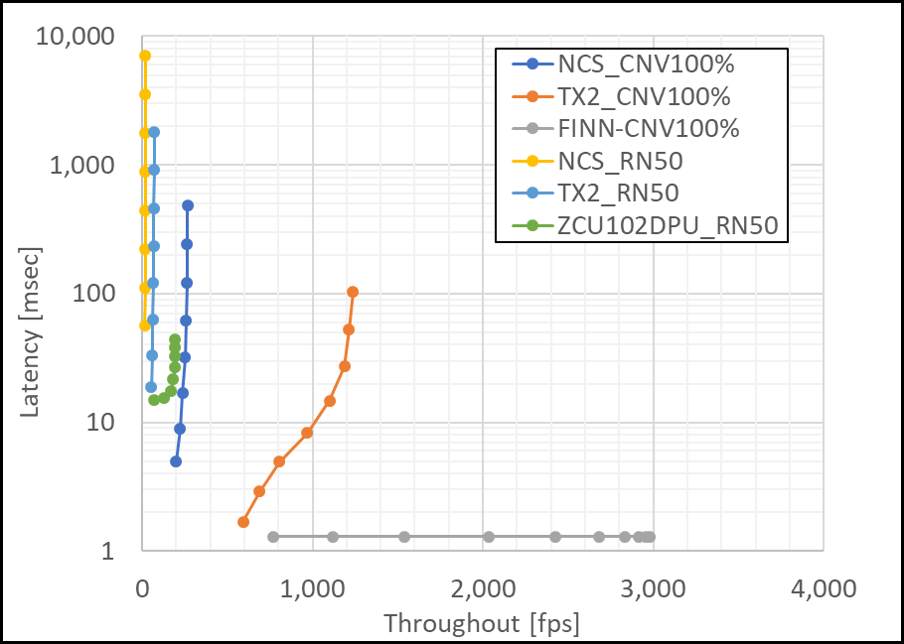
\includegraphics[width=0.6\linewidth]{figures/latency_behaviour.png}
% \caption{Latency versus throughput for different batch sizes, thread counts and stream sizes. For most architectures increasing the latter improves throughput at the cost of latency, with exception of spatial architectures, where latency remains constant.}
% \label{fig:latfps1}
% \end{figure} 

% \subsubsection{Other Considerations}
% Finally, we would also like mention different options in regards to form factors. There is a spectrum of form factors available for all of these accelerators and it is important as it poses additional challenges in regards to ensuring fair measurements.
% Cloud CPUs are only deployed in motherboard sockets, while GPUs and DPUs (including FPGA-based ones) are typically available in PCIe accelerator form factors. The motherboards hold significant amounts of additional circuitry, which prevents us from measuring power of CPUs in isolation.
% Further there are specialized AI machines such as Nvidia's DGX-1~\cite{dgx}, however their focus is mostly on training which is beyond the scope of this thesis.
% Similarly, the TPU is available in customized form factors, so called pods, for Google's data centers, and no power metrics are available.
% In the embedded space, we see many customized platforms. We believe it's useful to distinguish between USB accelerator options (which are further constrained to USB power budget of 2.5W), and socket-powered boards. Most of these boards are not actually intended as the final product, but more as development or evaluation boards. 
% The actually deployed form factor is heavily customized to the specific use case of the end customer. Similarly to the server space, depending on the complexity of the evaluation boards, power consumption might be inflated given collateral devices located on the same platform.

%%%%%%%%%%%%%%%%%%%%%%%%%%%%%%%%%%%%%%%%%%%%%%%%%%%%%%%%%%%%%%%%%%%%%%%%%%%%%%%%%%%%%%%%%%%%

\begin{table}[!ht]
\resizebox{\linewidth}{!}{
\begin{tabular}{|c||c|c|c|c|c|c|c|}
\hline
\textbf{Server-class} & \textbf{Throughput} & \textbf{Latency} & \textbf{Power} & \textbf{Ext. Mem. Bandwidth} & \textbf{HW specialization} & \textbf{Ease of Use} & \textbf{Training/Inference} \\
\hline \hline
\textbf{Conventional} & & & & & & & \\
CPU & Medium & High & High & Medium & Low & High & Both \\
DPU-MPE & High & Medium-High & Medium & High & Medium & Low-Medium & Inference \\
e.g. DPU-MPE (Gaphcore IPU) & Medium & Medium & Medium & High & Medium & Medium & Inference \\
DPU-Spatial & High & Low & Medium & High & High & Low & Inference \\
GPU (NVIDIA A100) & High & High & High & High & Medium & High & Both \\
\hline \hline
\textbf{Speculative} & & & & & & & \\
Cerebras CS-1 & Very High & Medium & High & Very High & Medium & Medium & Both \\
\hline
\end{tabular}}
\caption{Characterization of types of hardware based on important metrics -- these are used as input to Fig.~\ref{fig:hwcompare}.
\label{tab:hwcompare}}
\end{table}


\begin{figure}[h!]
\centering
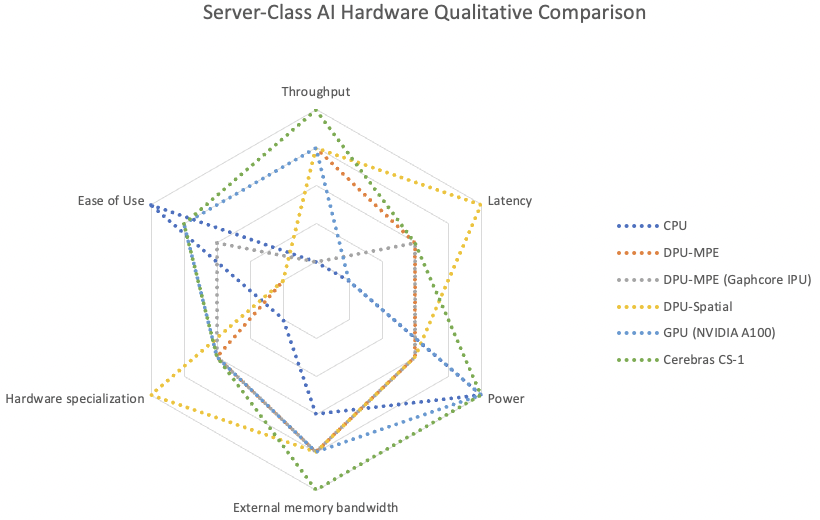
\includegraphics[width=0.8\linewidth]{figures/radar_chart.png}
\caption{Qualitative comparison of popular server-class hardware platforms.}
\label{fig:hwcompare}
\end{figure}

\textcolor{red}{[S.H. Table: seems strange to have two different MPU's listed.  Diagram - seems superfluous, since it has the same info as the table - I'd cut it.]}

\paragraph*{Summary of Conventional CMOS Hardware Architectures}

We analysed three categories of hardware architectures that are leveraged for CNN inference, namely common CPUs, SIMD based vector processors such as GPUs, and DPUs which are specialized architectures for acceleration of deep learning workloads. 
An overview of the architectures is visualized in Table~\ref{tab:hwcompare} and Figure~\ref{fig:hwcompare}.
Please note, "Ease of Use" includes compute kernel programmability as well as general ease of use.
Degree of specialization includes operators, precision support and customization towards topologies.
In summary, for DPUs, we distinguish between tensor processors which leverage a matrix of processing engines, and spatial architectures which can be further specialized for specific topologies using FPGAs.
CPUs are the most general solution but high in power. GPUs and DPUs offer the highest performance, though GPU are more expensive in energy cost. Spatial DPU architectures excel at low latency and provide the highest compute efficiency through maximized customization. 
CPUs, GPUs and DPUs (MPE) use a sequential layer-by-layer compute model whereas spatial DPUs execute all layers of the network concurrently. 
Hardened topologies in form of ASICs, CPU and GPU offer a fixed set of native dataypes, whereas FPGAs can adopt any precision and numerical representation, which provides the utmost flexibility and leverages optimization with quantization to the maximum, whereas hardened approaches need to default to the next higher supported precision into which the reduced precision variable can be embedded. However the programmability in the FPGA fabric also comes at a speed and energy cost.
All architectures can benefit from coarse-grained pruning optimization techniques. Only sparse execution engines can benefit from irregular pruning, such as synaptic pruning.
We also discussed the various deployment options. 
Many devices offer different power and operating modes as different compromises between throughput and power consumption to adapt to the potentially very different optimization targets of different application settings. Similarly, batch sizes, thread counts and stream sizes offer another compromise in regards to throughput versus latency. Again this is to facilitate a spectrum of different use cases.
Finally, the table shows that speculative approaches such as Cerebras can bring fundamental performance scalability.
Overall, each approach comes with its own advantages and disadvantages and the best solution greatly depends on the specifics of a given use case.

%\subsubsection{Conventional ML Hardware}
%\subsubsection{Emerging Beyond CMOS Hardware}
%%%%%%%%%%%%%%%%%%%%%%%%%%%%%%%%%%%%%%%%%%%%%%%%%%%%%%%%%%%%%%%%%%
\subsection{Hardware/Software Codesign Example: FPGA-based Systems}
\label{sec:codesign}

In the last decade we have observed the rise of two significant paradigms that have come to scientific applications: heterogeneous-computing systems and machine learning. Heterogeneous computing can overcome the decline of Moore's Law and Dennard Scaling and achieve the desired computational cost and performance by executing portions of the applications on the best-matched hardware, e.g., CPU, GPU, ASIC, and FPGA. On the other hand, machine learning is an automatic process that creates programs that can solve classes of problems. As with traditional programming, machine learning can significantly benefit from heterogeneous computing; in addition, designers can tailor specialized but reprogrammable hardware to fit ever-changing machine learning requirements. This section examines tools and methodologies that can automatically deploy and orchestrate machine learning on FPGA systems in larger scientific applications.  FPGAs are a particularly compelling example to explore because the efficiency of the hardware coupled with their programmability makes for an interesting case study in hardware/software codesign.   

Traditional software programming is complicated, and parallel high-performance programming is even more challenging. Programming heterogeneous systems that integrate FPGAs brings the challenge to the next level: the programmer must deal with a multi-objective optimization problem that involves performance and costs, i.e., hardware resources.
For machine learning applications, a common practice is to profile the application on CPU (or GPU) to identify the bottlenecks to be offloaded onto the reprogrammable logic to improve latency, throughput, or energy efficiency of the application as a whole. Then, part of the application can remain on the CPUs to control the execution and interact with the rest of the scientific setup.

\paragraph*{FPGA Programming}
FPGA are configurable integrated circuits that provide a good tradeoff in
terms of performance, power consumption, and flexibility with
respect to other hardware paradigms. However, it is a challenging and lengthy task to program FPGAs. FPGA programming has traditionally been a job for hardware designers familiar with digital design and computer architecture. These requirements lead to a steep learning curve for software developers and other domain experts. In order to lower the entry barrier, there has been a growing focus on designing FPGA hardware at a higher level of abstraction. As a result, various approaches have brought FPGA development into the mainstream by allowing developers to design for FPGAs at a higher level using familiar languages such as C, C++, OpenCL, and in some cases, even C\# \cite{kiwiHLS}. Here an important question arises: what are the additional advantages of designing the hardware at a higher level of abstraction? High-level languages (HLLs) include various constructs and design patterns that are more functionally expressive. Furthermore, the amount of time spent in the verification of the design is also a crucial factor. Hardware-description languages such as Verilog or VHDL focus on the final implementation details and, because of that, are more verbose. Bigger code repositories are not easy to verify for functional correctness. On the other hand, HLLs are more compact and simulate faster. Thus, a designer can do more verification in the same span of time. Despite these advances, FPGA programming remains complex. This has compelled academia and industry to develop new compilers, frameworks, and libraries to facilitate the hardware design.

\paragraph*{High-Level Synthesis and Languages}

High-level synthesis (HLS), also known as behavioral or algorithmic synthesis, is an automated design process that takes as input a functional description of a design and outputs an RTL implementation. It transforms an untimed (or partially timed) high-level specification into a fully timed implementation. The process of HLS starts by analyzing the data dependencies between the various operations in the functional description. This analysis leads to a Data Flow Graph (DFG) representation. After the DFG generation, during the allocation phase, HLS maps each operation onto a hardware resource with latency and area characteristics. Then, HLS adds the notion of time to the design during the scheduling phase. Scheduling takes the operations and resources of the DFG and decides in which clock cycle to execute them, given their latency information. This step infers sequential logic by adding registers between operations and creating finite state machines~\cite{hlsbluebook}. 

Over the past three decades, many HLS tools have been proposed. The work in \cite{survey_evaluation} presents an evaluation of different academic and commercial HLS tools tested on the same set of benchmarks. These tools have different input languages, perform different internal optimizations, and produce different quality results, even for the same input languages. The results show that each HLS tool can significantly improve performance once the designer has mastered benchmark-specific optimizations and constraints. However, academic HLS tools have a higher learning curve because of a minor focus on usability. Commercial HLS tools have an advantage because of their better documentation, robustness, and design verification integration.

In terms of input languages for HLS, most of the HLLs are variants of the C language. However, there are a few limitations to generate hardware from a pure C specification. First, C lacks the notion of timing and concurrency. The designer must rely on the HLS tool to create clock-based timing. Similarly, the designer must specify the concurrency model or rely on HLS to extract the parallelism among operations or processes. Second, C lacks bit-accurate data types. It only provides ``native'' data types such as \texttt{char}, \texttt{int}, and \texttt{long}, whose size is a multiple of a byte. Thirdly it lacks the concepts of hardware interfaces and communication channels. SystemC was adopted as HLS language to address all of these limitations~\cite{6838614}. However, SystemC still has not entirely made inroads in the FPGA community. Another common problem with all C-based languages, including SystemC, is memory access and modeling. These languages have a flat memory model, and memory access is done through pointers. Either HLS has to decide how to implement the memories in hardware, or the designer must leverage additional HLS directives or libraries to model the memory sub-system properly. Finally, in the family of the C-based specification languages for HLS, the SYCL language is emerging. SYCL (pronounced sickle) is an industry-driven standard that adds parallelism to C++ to design heterogeneous systems. SYCL programs perform best when paired with SYCL-aware C++ compilers such as the open-source data-parallel C++ (DPC++) compiler \cite{dpcplus}.

Apart from the variations of C, Bluespec is a language for the description and synthesis of hardware based on SystemVerilog. It provides levels of abstraction with a clean semantic that highlights aspects of the architecture. It can be considered a high-level functional HDL, where modules are implemented as rules using SystemVerilog syntax. Those rules are called guarded atomic actions and express behaviors as concurrently cooperating finite state machines (FSMs). Another recent language among FPGA designers is Chisel. It is based on Scala and supports hardware definition using highly parameterized generators, object-oriented and functional programming. Similar to an HLS flow, it compiles into an RTL Verilog implementation. 

\begin {table} [h]
	\begin{center}
		\caption {A brief taxonomy of domain-specific languages and frameworks for FPGA applications~\label{DSLs}}
		\begin{tabular}{ | l | l | l | p{0.1cm}|}
			\hline
			\textbf{Domain and Interfaces} &  \textbf{DSLs and Frameworks} \\ \hline  
			Signal-Processing &  HDL Coder, LabView, Spiral, VSIPL  \\            \hline
			Networking  &  SNORT \cite{snort}, Click, P4\\            \hline
			Databases & Glacier  \\ \hline
			Machine Learning & OptiML  \\ \hline 
			Numerics &Verilog
			AMS   \\            \hline
			Streaming & Maxeler, SCORE, Lime  \\            \hline
			Dataflow & OpenDF, OpenSpatial  \\            \hline
			Graphs & GraphStep, GraphGen  \\            \hline
			Data Parallel & MapReduce, Accelerator, FCUDA, Aetherling, SuSy  \\            \hline
			Circuit Generators & Flopoco, JHDL, PAMDC  \\            \hline
			Image processing & HIPACC, FROST, Darkroom, RIPL, PolyMage \\            \hline
 			Static &  JBits, TVM \cite{tvm}, TAPAS \\            \hline
				Dynamic &  PyRTL \cite{pyrtl}, APARAPI \cite{arapa}, TornadoVM\cite{tornado}, Caldeira, \\ & Lime,
		LINQits, DHDL, Spatial \\            \hline
		Type Systems & DAHLIA \\ \hline
		Verification & Kami \\ \hline
		Virtualization & Cascade \\ \hline
		\end{tabular}
	\end{center}
\end {table}

Although the languages mentioned above have helped create efficient hardware and significantly shorten the development time, specific coding techniques are still necessary. Also, the growth and diversification of the application domains have shown the limitations of these programming languages. This has further pushed the level of abstraction to domain-specific languages (DSLs). In recent years, we are observing the growth of a considerable corpus of DSLs and frameworks for FPGA design \cite{7577380, transparent}. In a DSL-based approach, the users and the tools can use domain knowledge to apply static and dynamic optimizations. However, a domain-specific HLS tool requires an appropriate compiler and a development environment that caters to the target domain. Table~\ref{DSLs} shows some of the DSLs and frameworks developed over the years for FPGA computing organized by domains of application. Although all the approaches in the table are diverse in terms of applications, the interesting question is, what are the common denominators? To the best of our knowledge, most of the approaches are broadly based on two approaches: either the DSL specification gets directly compiled into the RTL implementation, or the approach leverages source-to-source compilers. In the latter case, the DSL compiler produces an equivalent source code in a different programming language, for example, C++, for a more standard HLS flow. 

\paragraph*{Software and Hardware Integration}

Running an application on a microprocessor may be a more accessible approach than designing and running specialized hardware, but at the expense of poor performance and higher power costs. This dilemma often is paired with the hardware and software partitioning problem, also known as Hardware/Software codesign. It is the process of dividing an application between a microprocessor component (if any) and one or more custom hardware or co-processors components to achieve desired performance goals. Understandably there exists a plethora of research work in this area. The authors in \cite{rfu} have provided background information on notable aspects of older FPGA technologies and simultaneously explained the fundamental architectures and design methods for codesign. Furthermore, the work in \cite{microarchitecture} is another comprehensive study that aims to evaluate and analyze the microarchitectural characteristics of state-of-the-art CPU-FPGA platforms in depth. That paper covers most of the shared-memory platforms with detailed benchmarks.

Nonetheless, partitioning involves various design decisions, and it is generally considered a complex problem. One of the critical challenges is enabling higher design productivity and a more accessible way to use FPGAs for users unfamiliar with the underlying concepts. One way of doing this is to provide standardization and abstraction, usually supported and enforced by an operating system. Operating systems simplify the programming interface through an abstracted programming model.

\textcolor{red}{[S.H. This section is a but choppy, and needs smoothing.  Also odd to be exclusively Xilinx.]The two leading FPGA vendors, Xilinx and Intel, have their own solutions. The Xilinx Runtime Library (XRT) \cite{XRT} is implemented as a combination of userspace and kernel driver components. It supports both PCIe-based boards and MPSoC based embedded platforms. Similarly, Xilinx SDSoc \cite{sdsoc} and SDAccel \cite{sdaccel} became publicly available later in late 2015; the former works only on select boards of the Zynq family of FPGAs, the latter only on selected PCIe-based boards for OpenCL computing. Since 2020 Xilinx has introduced Vitis \cite{vitis} as a unified platform. Vitis Unified Software Platform is a comprehensive development environment to build and seamlessly deploy accelerated applications on Xilinx platforms, including on-premises Alveo cards, FPGA-instances in the cloud, and embedded platforms.}
%In addition, the recent efforts of Xilinx under the flagship Versal \cite{versal} is also a step towards codesign applications. Intel has the Open Programmable Acceleration Engine (OPAE) \cite{intelopae} which is the API library for programmers writing host applications that will leverage the FPGA acceleration. Likewise, Intel oneAPI \cite{inteloneapi} is an open, unified programming model built on standards to simplify the development and deployment of data-centric workloads across CPUs, GPUs, FPGAs, and other accelerators.

Apart from vendor solutions, academia and the open-source community have also attempted to simplify the integration of applications, operating systems, and hardware acceleration. For a comprehensive analysis, the reader is referred to the works in \cite{reconfig_os, connectal}, which give a historical review and summary on ideas and key concepts to include reconfigurable computing aspects in operating systems. They also present an overview of published and available operating systems of the last 30 years targeting reconfigurable computing. Similarly, the design exploration and engineering of FPGA drivers that are portable across multiple physical interfaces (PCIe, Ethernet, optical links) have remained a significant part of HW/SW codesign research. The challenges come from the variety of FPGA boards, the plethora of interfaces, and the diverse user requirements. Fundamentally, the FPGA drivers should allow the designer to load or reconfigure an application bitstream and support data transfers between the FPGA and host.

A significant engineering challenge is to consider how to partition driver functionality between the hardware and software components. One growing research focus is to exploit the spatial parallelism of FPGA technology through implementing multiple queues on FPGA drivers. A thorough analysis of system-level drivers for FPGA is out of the scope of our white paper. Readers interested in FPGA system-level drivers are referred to the work in \cite{fpga_drivers, fpgadrivers2}. The authors of those papers have provided benchmarks of various mainstream academic and vendor solutions regarding system-level drivers in the FPGA domain. 

Despite various existing OS and driver solutions, an open problem that remains is standardization. An industry-wide standardization would allow for faster development and better portability, and (re)usability of FPGA applications. There is already ongoing work in this area. Standards like the CCIX consortium \cite{ccix} and the Heterogeneous System Architecture (HSA) foundation \cite{hsa}  have already made good progress.

\paragraph*{The Case for ML Frameworks for FPGA Design}

Machine learning is one of the fastest growing application domains and over the years there has been an increasing demand of an established framework that caters to the needs of ML researchers and domain experts working with FPGAs. The main reason is the complexity of the traditional approaches that require significant engineering effort. Two main ML frameworks are making the effort to fill this vacuum: hls4ml and FINN. Considering the aforementioned tools, compilers, programming languages and co-design solutions, both hls4ml and FINN have the potential to reach a broader scientific community. \textcolor{red}{Add a description of FINN, while hls4ml has been described in Sec. 2.1.4}.

\textcolor{red}{[S.H. Need a section to wrap up 4.4.  Summary, conclusion, what have you.]}

%\textbf{FPGA supremacy for data acquisition and IO integration:}
%
%As presented before, each computing platform offers specific characteristics which suit a subset of applications. It is because the performance, efficiency, flexibility and ease-to-use are different sides of a multi parameter tradeoff. CPUs and GPUs placed at the extreme ease-to-use suitable for sequential and SIMD compatible algorithms, respectively. In contrast, ASIC implementations are efficient for any custom circuit at the cost of the lengthy and costly design process. FPGA chips place in the middle ground. Although they are not easy to be used, they offer customizable resources while delivering near-ASIC performance. These unique features make them suitable for fast prototyping and deployment for low-volume production, especially when the final circuit is not known beforehand, as it is the case in many DNN-powered applications \cite{10.1145/3411757.3411759}. 
%
%FPGA technologies also uniquely offer flexible IO integration, a game-changer for many high-performance and low-latency applications. This is an optimization opportunity where the communication between the compute units and data sources/sinks dictates the performance boundaries. These architectures provide hundreds of General purpose IOs backed by customizable hard/soft IP cores and the required analog circuits. As this flexibility requires rewiring the PCB boards, standard high-throughput connectors, such as FPGA Mezzanine Card (FMC) connectors, are developed, enabling the necessary flexibility via daughter board expansion, as fast as 40 Gb/s for the FMC case~\cite{WP_Xilinx_FMC}. The chance of efficient data acquisition bypasses the intermediary off-chip memories, which is inevitable for CPU/GPU/TPU-like systems. The followings are the major application categories which benefited the most from the mentioned features.
%
%{\bf High-performance computing (HPC)}: Dealing with large workloads, the received data can be moved/fetch to/from memory, while techniques like double buffering hide the data movement effects on throughput. However, this poses a significant extra amount of latency delay to the process. As measured by \cite{10.1145/3230543.3230560}, for a PCI-express-based network interface card (NIC), the contribution of PIC-express link to the total latency is in the range of 77-90\%. But, for small loads, in which latency is a constraint, data movement is not tolerable. Network function virtualization (NFV) is one great example where a massive number of user requests should be addressed quickly every second. This is possible by coupling FPGA to CPU caches to use these fast and close-to CPU memories as an intermediary for communication purposes \cite{10.1145/3411757.3411759}.
%
%{\bf Sensing}: These applications require analog to digital (ADC) or visa versa conversion, which deployment of them is always a challenge, especially for high resolution and/or high sample rate sensors/actuators. However, this is possible by connecting ADCs/DACs directly to the compute unit using FPGA IOs. Beyond that, the new FPGA architectures provide required analog circuits inside the chip for direct RF sampling from the transceivers toward having a practical reconfigurable system on a chip (SoC), such as Xilinx RFSoC series \cite{DBLP:conf/isscc/VazLVLMBMKTMBEF17,WP_Xilinx_RF}. The most recent versions, Zynq UltraScale+ RFSoC ZU48DR, integrates eight 14-bit 5GSPS ADCs, eight 14-bit 10GSPS DACs \cite{WP_Xilinx_ZCU208}. These RF class DAC/ADC circuits join FPGA compute resources to deploy ML-powered software-defined network applications such as \cite{DBLP:conf/ipps/TridgellBLKK020}. In a more scientific application, this integration enables Gas electron multiplier (GEM) detectors with 128 channels of 16bit data at 80M sample/second, which is a transfer 20.48GB/s \cite{GEMDetectors}. 
%
%{\bf Network monitoring}: In Cybersecurity and network management applications, high-throughput flows of packets should be analyzed, preferably without adding notable latency. Consequently, the extra latency of data movement is not acceptable. FPGA technology makes it possible by offering a wide range of IPs suitable for both of the application extremes; low cost and high speed. State of the art Xilinx Versal ACAP FPGAs incorporates on-chip 100G Multi rate Ethernet MACs, which is dynamically switchable to 10G, 25G, 40G, 50G, and 100G rates \cite{DBLP:conf/fpga/GaideGRB19}.
%
%Digital Signal processing: Although DSP applications map well to GPU systems, again, when the latency budget is low, FPGA boards could be the solution. FPGA supremacy becomes clearer by enabling more optimization techniques such as quantization and sparse computing, which requires customizing the data paths. The mentioned flexible IO integration also enhance the latency suitable for applications such as realtime signal decoding and compression \cite{WP_Xilinx_decoder}. 
%
%Although the mentioned features make FPGA an exciting platform, historically, when the applications become more mature, the ASIC designs replace them due to their efficiency and mass production costs. As computer architecture research show, FPGA paradigm is a key to future computer architecture \cite{10.1145/3411757.3411759}. However, the current architectures do not position correctly on the performance-customizability tradeoff range. Future FPGAs will include more hardened coarse-grained compute units and larger memory blocks with less flexibility. It is mainly because of the workload shift as the result of the dominancy of ML-powered applications. It is also predictable, that future computers incorporate a wide range of resources from CPU, GPU, FPGA architectures and efficient customized ASIC units all to gather as an SoC to efficiently address each aspects of the future implementations \cite{10.1145/3411757.3411759}. 
%
%%[source-1] = GEMDetectors 
%%[source-3] = DBLP:conf/isscc/VazLVLMBMKTMBEF17
%%[source-4] = WP_Xilinx_RF 
%%[source-5] = WP_Xilinx_FMC 
%%[source-10] = WP_Xilinx_ZCU208
%%[PCI-Express] = 10.1145/3230543.3230560
%%discuss = [10.1145/3411757.3411759]
%
%
%%\textbf{Rob's items:}
%%\begin{itemize}
%%    \item Specialized hardware for specialized purposes
%%    \item Some history of heterogeneous efforts?
%%    \begin{itemize}
%%        \item Sh/RapidMind
%%        \item Brook
%%        \item Accelerator
%%    \end{itemize}
%%    \item Rise of CUDA and ever more generally programmable NVIDIA hardware
%%    \item Rise of OpenCL
%%    \item Pragma/Directive-based language extensions with OpenMP and OpenACC
%%    \item SYCL and standard C++
%%    \item Reduced precision and non-standard types
%%    \item Rise of specialized separate hardware for inference and training.
%%\end{itemize}
%
%\textbf{SEDA's items:}
%\begin{itemize}
%    \item tightly coupled CPU-FPGA accelerator systems - a quick overview 
%    \item Intel's System on Module 
%    \item \textbf{OpenCL programming paradigm:} OpenCL~\cite{munshi2009opencl} is a programming model and standard from the Khronos Group for running applications across heterogeneous platforms. It provides a top-level abstraction for low-level hardware routines, memory consistency, and parallel execution models, thus enables application acceleration on heterogeneous systems. An OpenCL-based application is consist of two parts. One is the \textit{host} code that executes on the host CPU. It can be written in any programming language and a commonly used one is C/C++ language. The other part is a C-based \textit{kernel} code that runs on the accelerator. The necessary APIs are provided by OpenCL to control the communications between the host CPU and the accelerator. The typical operation flow in OpenCL is that the host processor first allocates all needed data in its own memory and prepares corresponding inputs to the kernel. The data is then transferred to the device memory via OpenCL APIs. The kernel is loaded and executed on the device. The output data of the kernel is written into device memory. The host waits the kernel execution to completion and transfers the kernel's output data from the device memory back to the host memory. 
%    \item \textbf{Intel FPGA SDK for OpenCL:} Intel provides an offline compiler called Intel FPGA SDK for OpenCL (AOC) to automate the process of transformation from high-level OpenCL description to the FPGA executable binary. This tool reduces the traditional HDL design complexities on FPGAs. Besides, often times the algorithm underlying the application needs to be revised and modified. Updating HDL code is time consuming and error prone, while this process is much more practical with AOC.  AOC first converts OpenCL code to LLVM intermediate representations (IRs), applies various optimizations and generates Verilog/VHDL output. The compiler leverages pre-written IP modules, like FIFO, load store unit, as well as the interface to global memory while generating the HDL code. In this flow, Intel Quartus, an FPGA design software, is used to perform synthesis, placement and routing to generate the final FPGA bitstream. 
%    An overview of the OpenCL architecture for FPGAs is shown in Figure~\ref{fig:opencl}. A CPU-based host is connected to the FPGA to configure the kernel execution via PCI-e bus. There can be multiple kernel pipelines (i.e., \textit{compute units}) for an OpenCL kernel. Each compute unit executes the OpenCL program in a pipelined fashion. In addition to the kernel pipeline, there are interfaces to internal and external memory. The internal memory includes two layers. First, the \textit{private memory}, storing private variables or small data structures for each work item, is constructed using parallel registers. Second, each compute unit can connect to \textit{local memory}, which utilizes on-chip high bandwidth block RAMs. The external memory, also called the \textit{global memory}, is shared between all kernel pipelines via a single global interconnect structure. It is often implemented in DRAM. Thus, accessing internal memory is much faster than global memory.
%
%\begin{figure*}[!t]
%\centering
%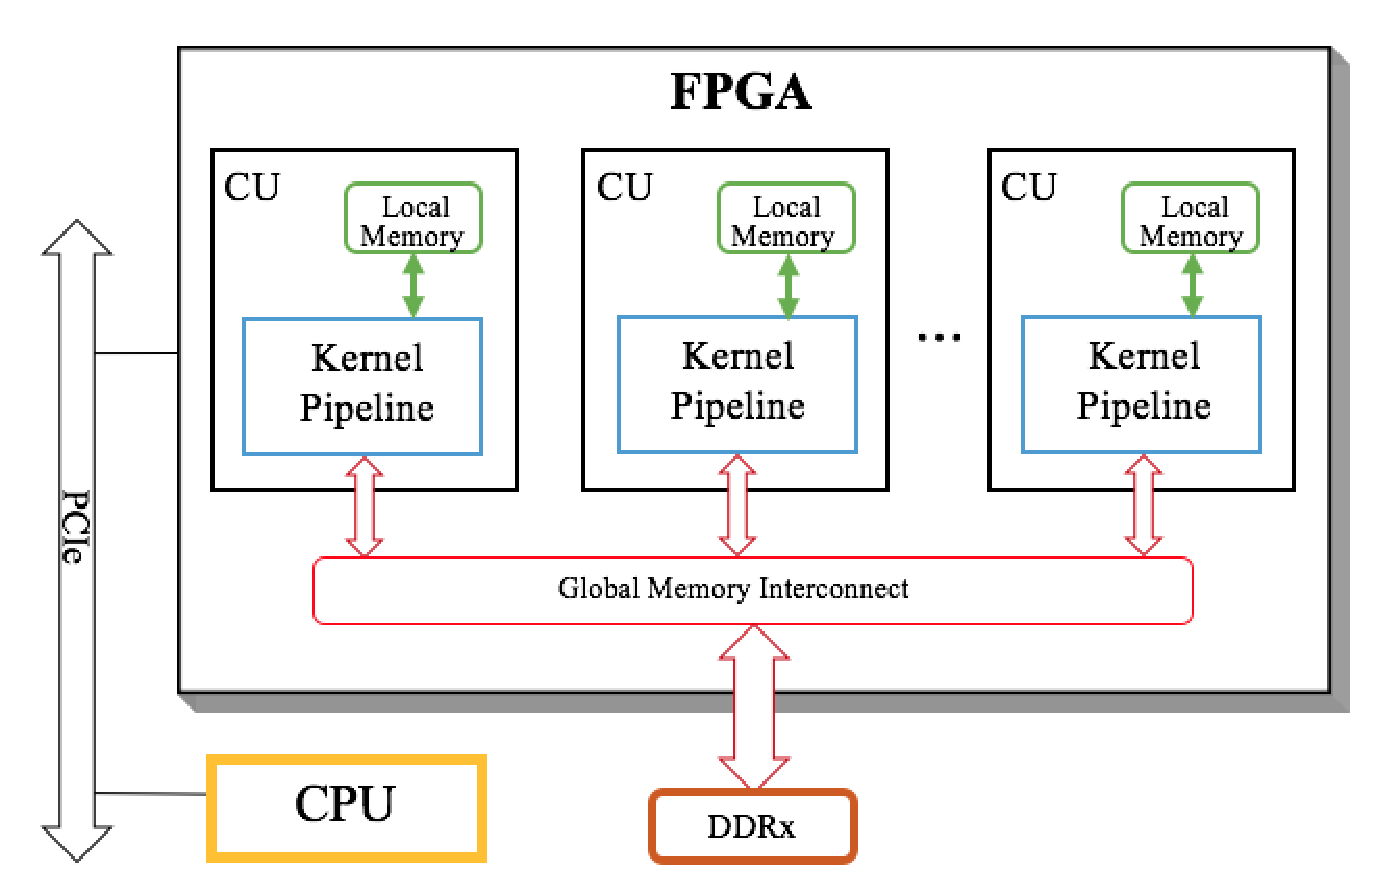
\includegraphics[width=0.70\textwidth]{figures/programingModel.eps}
%\caption{OpenCL architecture for FPGAs}
%\label{fig:opencl}
%\end{figure*}
%    
%    
%    
%\end{itemize}
%
%
%\textbf{GPU}
%\begin{itemize}
%    \item CUDA, OpenCL
%\end{itemize}

%%%%%%%%%%%%%%%%%%%%%%%%%%%%%%%%%%%%%%%%%%%%%%%%%%%%%%%%%%%%%%%%%%
%%%%%%%%%%%%%%%%%%%%%%%%%%%%%%%%%%%%%%%%%%%%%%%%%%%%%%%%%%%%%%%%%%
\subsection{Beyond-CMOS neuromorphic hardware}
\label{sec:beyondcmos}

With rapidly growing machine learning (ML) applications comes the acute need for their efficient hardware implementations. Most of the efforts are focused on digital CMOS technology, such as implementations based on general-purpose TPUs/GPUs, FPGAs, and more specialized ML hardware accelerators.  The steady improvements in such hardware platforms' performance and energy efficiency over the past decade are attributed to the use of very advanced, sub-10-nm CMOS processes and holistic optimization of circuits, architectures, and algorithms.  It includes, for example, taking advantage of aggressive voltage supply scaling \cite{Moons2017}, very deep pipelines and extensive data reuse in architectures \cite{Chen2017}, and lowering the precision of weights and activations of the algorithms \cite{Simons2019}.  As a result, very compact state-of-the-art neural networks, such as MobileNet based on 3.4M parameters and 300M multiply-and-add operations per inference \cite{Sandler2018}, can now be fitted entirely on a single chip. However, on all these fronts, advances are saturating and cannot rely on the faltering Moore's law. 

On the other hand, further progress would be essential because ML algorithms are getting increasingly more complex. For example, transformer networks \cite{Vaswani2017}, the state-of-the-art approach for many ML tasks today \cite{Vaswani2017, Vinyals2019, Dosovitskiy2020}, could have hundreds of billions of parameters and perform hundreds of trillions of operations per inference. Moreover, the transformer's functional performance typically improves with the model size \cite{Rajbhandari2020,Brown2020}. Training such models requires enormous, data-center-scale (e.g., kiloTPU-year) resources, while performing inference on resource-constrained edge devices would be extremely challenging. 

The opportunities for building more efficient hardware may come from biological neural networks. Indeed, it is believed that the human brain, with its $>$1000$\times$ more synapses than the weights in the largest transformer network, is extremely energy efficient \cite{Hasler2013}, which serves as a general motivation for developing neuromorphic hardware \cite{Mead1990}. There is a long history of CMOS neuromorphic circuits \cite{Indiveri2011}. However, unleashing the full potential of neuromorphic computing might require novel, beyond-CMOS device and circuit technologies \cite{Berggren2020} that allow for more efficient implementations of various functionalities of biological neural systems. 

In this section, the most prominent emerging technology proposals, including those based on emerging dense analog memory device circuits, are grouped according to the targeted low-level neuromorphic functionality - see, e.g. reviews in \cite{Burr2017, Bavandpour2018, Yang2013NatureNano, Yu2018IEEE} and original work utilizing volatile \cite{Sheridan2017, Cai2019NatElec, Chu2014Neuro, Yeon2020, Ohno2011, Wang2017NatMat, Pickett2013, Wang2018NatElec, Zhang2018Small, Lashkare2018, Adda2018} and nonvolatile \cite{Alibart2012, Adam2017,Govoreanu2013, Prezioso2015, Prezioso2016, Prezioso2018, MerrikhBayat2018, Lin2020NatElec, Hu2018AdvMat, Yao2020Nature, Liu2020ISSCC, Kim2019XBAR, Cai2020NatElec, Mahmoodi2019IEDM, Mahmoodi2019NatComm, Li2016IEDM, Wang2018NatElec, Pedretti2017}  memristors, phase change memories (PCM) \cite{Burr2015, Tuma2016, Ambrogio2018, Karunaratne2020, Joshi2020, Kuzum2011, Rios2019}, and nonvolatile NOR \cite{Guo2017CICC, Guo2017IEDM, MerrikhBayat2015, Mahmoodi2019NatComm}, and NAND \cite{Bavandpour2019NAND, Bavandpour2020, Lee2019NAND}, and organic volatile \cite{Fuller2019} floating gate memories, as well as multiferroic and spintronic \cite{Grollier2020, Ostwal2018, Sengupta2016, Romera2018, Ni2018IEDM}, photonic \cite{Shasti2021, Goi2020, Rios2019, Lin2019Sciece, Hamerly2019PhysRevX, Hamley2019, Shen2017NatPhot, Tait2016, Feldmann2019, Buckley2017, Bruiner2013, Vandoorne2014}, and superconductor \cite{Segall2017, Buckley2017, Rowlands2021} circuits. More discussion is devoted to analog vector-by-matrix multiplication circuits in the following subsection because of their immediate value for today's state-of-the-art algorithms. More biologically-realistic proposals described in the subsequent sections are less emphasized because they target algorithms with inferior performance. The least mature though very intriguing quantum neuromorphic computing \cite{Yamamoto2020, Markovich2020} is not discussed in this brief review.
    

\paragraph*{Analog Vector-by-Matrix Multiplication}

The emergence of dense analog-grade nonvolatile memories in the past two decades renewed interest in analog-circuit implementations of vector-by-matrix multiplication (VMMs) \cite{Mead1990, Holmes1993, Alibart2012, Widrow1962, Chawla2004, Guo2017CICC, MerrikhBayat2015}, which is the most common and frequently performed operation of any neural network in training or inference \cite{Hertz1991, Gerstner2002}. In the simplest case, such a circuit is comprised of a matrix of memory cells that serve as configurable resistors for encoding the matrix (synaptic) weights and peripheral sense amplifiers playing the role of neurons (Fig. \ref{fig:VMM}). The input vector is encoded as voltages applied to rows of the memory matrix so that the currents flowing into virtually grounded columns correspond to VMM results. Because addition and multiplication are performed on the physical level, via Kirchhoff's and Ohm's laws respectively, such an approach can be extremely fast and energy-efficient, provided that memory devices are dense and their conductances are adjustable (i.e., multi-state). The energy efficiency in part comes from performing ``in-memory" computing that reduces the amount of data (corresponding to the synaptic weights) that are moved across or in-and-out of the chip during computation. Such communication overhead could dominate the energy consumption in the most advanced digital CMOS implementations.

\begin{figure}[!t]
\centering
\includegraphics[width=0.30\textwidth]{figures/vmm.png}
\caption{Analog vector-by-matrix multiplication (VMM) in a crossbar circuit with adjustable crosspoint devices. For clarity, the output signal is shown for just one column of the array, while sense amplifier circuitry is not shown. Note that other VMM designs, e.g. utilizing duration of applied voltage pulses, rather than their amplitudes, for encoding inputs/outputs, are now being actively explored – see, e.g., their brief review in Ref. \cite{Bavandpour2018}}.
\label{fig:VMM}
\end{figure}

The general challenge towards practical adoption of such circuits, especially when using the most prospective emerging memory technologies, is variations in $I$-$V$ characteristics, e.g., in the switching voltages applied to change the memory state.  In light of this challenge, the most straightforward application is ex-situ trained inference accelerators for the earlier firing-rate neural networks \cite{Bavandpour2018}, i.e., the so-called second generation of artificial neural networks (ANNs) with graded-response neurons. In such applications, memory devices are updated infrequently, only when new inference functionality should be programmed. Thus, crosspoint devices' conductances can be tuned with slower, more tolerant to device variations write schemes. For example, after the weights have been found in the software, memory cells are programmed, one by one, using feedback write-verify algorithms that can adapt to the unique $I$-$V$ characteristics of each device \cite{Alibart2012}.  For the same reason, the switching endurance, i.e., the number of times the memory devices can be reliably programmed, and the write speed/energy are less critical.  Additionally, VMM operations in the inference of many neural networks could be performed with moderate, less than 8-bit precision, without incurring accuracy loss \cite{Yang2019IEDM}, which further relaxes requirements for analog properties and permits more $I$-$V$ non-idealities and noise.

The most advanced neuromorphic inference circuits have been demonstrated with more mature floating-gate transistor memory circuits. Up until recently, such circuits were implemented primarily with ``synaptic transistors" \cite{Diorio1996}, which may be fabricated using the standard CMOS technology, and several sophisticated, efficient systems were demonstrated \cite{Hasler2013, Chawla2004, George2016}.  However, these devices have relatively large areas ($>$10$^3$ $F^2$, where $F$ is the minimum feature size), leading to higher interconnect capacitance and hence larger time delays. More recent work focused on implementing mixed-signal networks with much denser ($\sim$40$F^2$) commercial NOR-flash memory arrays redesigned for analog computing applications \cite{MerrikhBayat2015, Guo2017CICC}. For example, a prototype of a 100K+-cell two-layer perceptron network fabricated in a 180-nm process with modified NOR-flash memory technology was reported in Ref. \cite{Guo2017IEDM}. It performed reliably, with negligible long-term drift and temperature sensitivity, and reproducible classification of the MNIST benchmark set images with $\sim95\%$ fidelity and sub-1-$\mu$s time delay and sub-20-nJ energy consumption per pattern. The energy-delay product was six orders of magnitude better than the best (at that time) 28-nm digital implementation performing the same task with a similar fidelity \cite{Guo2017IEDM}. 

Recent theoretical studies showed that neuromorphic inference circuits could be also implemented with much denser 3D-NAND flash memories \cite{Bavandpour2019NAND, Bavandpour2020, Lee2019NAND}, projected to scale eventually to 10 terabits per square inch density. In the long term, the most promising are perhaps circuits based on metal-oxide resistive switching random access (ReRAM for short, which are also called metal-oxide memristors) \cite{Yang2013NatureNano, Yu2018IEEE}, especially their passively integrated (0T1R) technology variety \cite{Kim2019XBAR}. Indeed, due to the ionic switching mechanism, ReRAM devices with dimensions below 10 nm still retain excellent analog properties and year-scale retention \cite{Govoreanu2013}. Furthermore, a low-temperature fabrication budget allows monolithic vertical integration of multiple ReRAM crossbar circuits, further increasing effective density \cite{Adam2017}. There has been rapid progress in scaling up the complexity of ReRAM-based neuromorphic circuit demonstrations over the past several years \cite{Prezioso2015, MerrikhBayat2018, Lin2020NatElec, Hu2018AdvMat, Yao2020Nature, Liu2020ISSCC, Kim2019XBAR}. However, the ReRAM technology is still in much need of improvement. In addition to high device variations, another remaining issue is high write currents and operating conductances, which must be decreased by at least one order of magnitude to reduce the significant overhead of peripheral circuits \cite{Kim2019XBAR}.

The device requirements for training hardware accelerators are different and much more stringent. For instance, the long retention is not required because weights are frequently updated. That allows using volatile memories in analog VMM circuits, such as interfacial memristors based on electron trapping/detrapping switching \cite{Sheridan2017, Cai2019NatElec, Chu2014Neuro} and solid-state-electrolyte memories \cite{Fuller2019, Yeon2020, Berggren2020}, or even capacitor-based memories controlling current via crosspoint transistors \cite{Ambrogio2018}. However, the toughest challenge is much higher computing and weight precision required for training operation and the need for efficient schemes for weight updates, which in turn necessitate drastically tighter device variations. The additional related requirement is that the change in device conductance upon applying the write pulse should not depend on its current state (the so-called linearity of update property). Otherwise, accurate conductance adjustment would require sending a unique write pulse based on the current device state, which would be hardly compatible with fast (in parallel) weight update. 

Phase change memories have also been investigated as candidates for variable resistors in analog VMM circuits \cite{Burr2015, Joshi2020}, though their main drawback is significant drift in the conductive state over time. High write endurance, high density (with vertical 3D-NAND-like integrated structure), and long retention are demonstrated in 1T Ferroelectric RAM devices. There is much excitement about such devices' applications in training and inference accelerators \cite{Ni2018IEDM}, though their analog properties are probably inferior to ReRAM.  The significant drawbacks of magnetic devices, such as magnetic tunnel junction memories, are smaller on/off current ratios, insufficient for practical VMM circuits, and poor analog properties for scaled-down devices \cite{Grollier2020}. 

The potentials of using light for implementing fast and large-fanout interconnect and linear computations, such as multiply-and-add operation, have motivated photonic neuromorphic computing research \cite{Berggren2020,Goi2020,Shasti2021,Hamley2019}. Different implementation flavors, e.g., with fixed \cite{Lin2019Sciece} and programmable \cite{Rios2019, Hamerly2019PhysRevX, Shen2017NatPhot, Tait2016} functionalities, have been recently suggested in the context of modern neural networks. Specifically, Ref. \cite{Lin2019Sciece} reports a system of multiple 3D-printed optical layers, each being a mesh of regions (neurons) with specifically chosen transmission-reflection properties, which can perform pattern classification inference similar to the convolutional neural networks. By sending a coherent light with amplitude-encoded input, a useful computation is performed at the speed of light. Specifically, the light diffracts and interferes when passing through the optical system and is ultimately steered to the specific region at the output layer corresponding to the pattern class. \cite{Rios2019, Hamerly2019PhysRevX, Shen2017NatPhot, Tait2016} report optical neuromorphic systems with configurable weights. The inputs are encoded in the light's energy, and the weights are encoded by optical attenuation in PCM devices in Ref. \cite{Rios2019} so that a product is computed by passing the light via PCM device. Ref. \cite{Tait2016} proposes encoding inputs with light amplitude and uses specific frequency for different VMM inputs. The light from inputs is combined and passed to the frequency selective weight banks based on a microring resonator (MRR) that features metal heaters to perform multiplication. In particular, the MRR coupling (i.e., weight) is controlled via heating by adjusting currents supplied to each MRR. In these reconfigurable implementations, the product accumulation (i.e., the summation operations in the VMM) is performed by integrating the light-induced charges on the photodetector. A very aggressive time-division multiplexing scheme for calculating VMM in which both weights and inputs are encoded in the coherent light's amplitude is proposed in Ref. \cite{Hamerly2019PhysRevX}. At one step of such scheme, the input light is fanned out into $n$ channels and combined with the light-encoded $n$ weights using a beam splitter and then sent to $n$ homodyne photodetectors to compute $n$ products in parallel. All-optical feed-forward inference based on Mach-Zehnder interferometer meshes utilizes single-valued decomposition for the weight matrix \cite{Shen2017NatPhot}. Unitary matrix transformations are implemented with optical beam splitters and phase shifters, while the diagonal matrix is implemented with optical attenuators. 

In principle, sub-aJ energy and sub-ps latency for a single multiply-and-add operation might be possible with optical computing \cite{Hamley2019}. However, the main challenge remains much large dimensions of the optical components and the very high I/O overhead of converting to and from optical domains \cite{Berggren2020, Shasti2021, Hamley2019}. The designs that rely on conversion to the electrical domain would be especially affected by poor integration density of optical devices due to larger electrical communication overheads, which were shown to overwhelm system-level performance of (much denser) ReRAM based circuits \cite{Bavandpour2018}. Optical systems would ultimately benefit from very wide ($\gg$10,000) dot-products and/or utilizing deep time-division multiplexing to amortize the I/O overhead. However, the possible issues of nonlinearities in charge integration and utility of such wide dot-product computations remain unclear \cite{Hamley2019}.  

\paragraph*{Stochastic Vector-by-Matrix Multiplication}

Computations performed by the brain are inherently stochastic, in that, e.g. substantially different neural responses are observed to the repeatable presentation of identical stimuli \cite{Rolls2010}. Such noisy operation is mimicked by probabilistic neural networks, such as Boltzmann machines \cite{Hinton1983} and deep belief neural networks \cite{Hinton2009}. In the simplest case, such a network is comprised of binary neurons that compute stochastic dot products, i.e., probabilistically generate output according to their pre-activation (dot-product) values. 

The stochastic functionality can be realized at either the synapse or the neuron side. In the latter, more straightforward scenario, the neuron first computes a dot-product of its inputs and corresponding weights deterministically. The result is then passed to some ``probabilistic" activation function, e.g., used as an argument in the sigmoid probability function, to determine the probability of generating high output. Because of the typically large ($>$100) ratio of synapses to neurons, the efficient deterministic dot-product implementations, e.g., with the already discussed analog VMM circuits, is of primary importance for realizing high-performance probabilistic neural network hardware. Still, earlier work showed that even the simplest, deterministic neurons may incur substantial overhead, e.g., occupy up to $30\%$ of the area and consume up to $40\%$ of energy for some neural network models \cite{Bavandpour2018}. Hence neuromorphic hardware would also benefit from the efficient realization of stochastic neurons.

Emerging devices can be broadly employed in two ways to achieve stochastic functionality, namely by using either dynamic or static $I$-$V$ characteristics of memory devices. Specifically, the former approach is to utilize intrinsically stochastic switching between memory states in emerging memory devices. For example, in MTJ memories, thermal fluctuation causes stochastic transition between the low resistance parallel and high resistance antiparallel states so that the probability of the final memory state upon switching could be controlled by the spin-torque current \cite{Grollier2020}. The melt-quench-induced reconfiguration of the atomic structure is intrinsically stochastic in phase-change memories (PCMs) \cite{Tuma2016}. These phenomena were suggested for implementing MTJ \cite{Ostwal2018} and PCM \cite{Tuma2016} stochastic neurons. The second approach is to utilize intrinsic and extrinsic current fluctuations in memory devices, e.g., random telegraph \cite{Cai2020NatElec} and thermal noise \cite{Mahmoodi2019IEDM} in ReRAM devices, or shot-noise in nanoscale floating gate transistors \cite{Mahmoodi2019IEDM, Mahmoodi2019NatComm}. In such an approach, the noisy current flowing into the neuron is compared against a reference value, e.g. using a simple latch, to implement a probabilistic activation function \cite{Mahmoodi2019NatComm}. 

The primary concern for the former approach is the limited endurance of many memories and the drift in the stochastic switching properties upon repeated switching. An additional drawback is a necessity for the co-integration of multiple memory device technologies for scalable stochastic dot-product circuits, e.g., integrating ReRAM-based artificial synapses and MTJ-based neurons. On the other hand, analog circuits based on ReRAM devices only (Fig. \ref{fig:VMM}), though operating at a much lower signal-to-noise ratio (SNR), can be utilized to implement stochastic VMM of the second approach. Furthermore, adjusting read voltage in such a circuit allows controlling SNR. Hence, the control of effective temperature, i.e. the slope of sigmoid probability function, enables efficient implementation of stochastic annealing in Boltzmann machines during runtime. The second approach's possible downside is slower operation because of lower read currents (which can be potentially addressed by utilizing external noise instead \cite{Mahmoodi2019NatComm}). Finally, the impact of noise quality on functional performance is another common concern. This issue has not been systematically studied yet, though Gaussian-like thermal or shot noise should be more advantageous for truly random operation.


\paragraph*{Spiking Neuron and Synaptic Plasticity}

Despite much recent progress in algorithms \cite{Neftci2019, Tavanaei2019}, the most biologically plausible, spiking neural networks (SNNs) \cite{Gerstner2002} are still inferior in the functional performance to simpler ANNs. If simpler ANNs would remain superior, the work of efficient SNN hardware could still be justified by the need to efficiently interface to the brain and/or model it, which in turn could lead to the development of higher-cognition artificial intelligence algorithms. An additional intriguing feature of SNNs is local weight update rules, requiring only information from pre- and post-synaptic neurons that could enable large-scale neuromorphic hardware with real-time training capabilities \cite{Thakur2018}. 

In the simplest SNN models, the information is encoded in spike-time correlations \cite{Gerstner2002}, while the network function is defined by the synaptic weights, which are adjusted based on the relative timing of spikes that are passed via synapses. In addition to VMM, the essential operations in SNNs are leaky-integrate-and-fire (LIF) function performed by neurons and various types of synaptic plasticity, such as short-term plasticity (STP) and long-term potentiation (LTP), and spike-timing-dependent-plasticity (STDP) \cite{Gerstner2002}. LIF neurons mimic the dynamic processes in the neuronal membrane, while synaptic plasticities mimic learning and memory mechanisms in biological networks. For example, STP is a temporary change in the synaptic strength implementing a short-term memory. Without immediate reinforcement of synaptic weight adjustment, the memory would be lost, i.e., the synaptic weight would relax to the original equilibrium state. On the other hand, the frequently repeated spiking stimulus causes long-term memory, e.g., permanent potentiation via the LTP mechanism. STDP is a time-dependent specialization of Hebbian learning. Its specific goal is to strengthen the synaptic efficiency when pre- and post- synaptic spikes happen in the expected causal temporal order and weaken it otherwise. 

A compact implementation of LIF neuron with biological, ms-scale integration times using conventional circuit technology is challenging because of the large capacitors that are required. Leaky integration circuits utilizing volatile memristors (e.g., based on filamentary \cite{Zhang2018Small}, interfacial \cite{Lashkare2018}, and Mott insulator \cite{Adda2018} switching mechanisms) have been suggested to address this problem. In such implementations, the integrated current is encoded with a conductive state of the volatile memory device. Neuron spiking functionality was demonstrated with threshold-switching (volatile) memory devices that feature S-type negative differential resistance (NDR) $I$-$V$ characteristics \cite{Pickett2013}. This approach's general idea is similar to the oscillator circuits based on S-type (NDR) device connected to a resistor-capacitor circuit \cite{Kesim2019}. LIF neurons based on spin-torque magnetic memories were simulated in Ref. \cite{Sengupta2016}. In such a neuron,  spin-torque oscillations are employed to generate spikes, while incremental magnetization and its relaxation mimic integration and leakage, respectively.

STP to LTP transition has been emulated with solid-state-electrolyte devices – see, e.g., original work in \cite{Ohno2011} and more recent work on ``diffusive" memristors \cite{Wang2017NatMat}. Specifically, the short and infrequent write pulses result in the formation of thin filaments, which are unstable and quickly dissolve, representing a short memory. However, a thicker and more stable filament can be formed by applying repeated and/or longer write pulses, thus mimicking transition to the LTP.  Different STDP window implementations, e.g., using PCM \cite{Kuzum2011} or metal-oxide ReRAM \cite{Prezioso2016} devices, have been suggested by carefully selecting the shape of pre and post-synaptic voltage pulses – see a comprehensive review of the emulated synaptic plasticity with memristive devices in Refs. \cite{Serrano-Gotarredona2013, Saighi2015}.

Several small-scale spiking neuromorphic systems based on emerging device technologies were demonstrated, including coincidence detection via STDP mechanism based on metal-oxide memristors \cite{Prezioso2018, Pedretti2017} and temporal data classification with diffusive memristors \cite{Wang2018NatElec}.  However, the overall progress in such advanced hardware has been much slower compared to simpler ANNs inference accelerators. The main reason is more demanding functionality from emerging devices in such applications and hence the more severe impact of device variations on the SNN operation and performance. For example, SNNs rely on fixed-magnitude spikes to update the conductance of multiple devices in parallel. Because of that, change in the conductances could vary drastically even with minor variation in $I$-$V$'s switching voltages, which in turn leads to very significant variations in STDP characteristics \cite{Prezioso2018}. On the other hand, implementation of simpler ex-situ trained ANNs is much less challenging because the write amplitude voltages in such networks can be adjusted uniquely for each device based on the feedback information during conductance tuning \cite{Alibart2012}. 

Superconductor circuits, e.g., based on rapid single flux quantum (RSFQ) variety \cite{Likharev1991}, are naturally suited for spiking circuits due to information encoding in SFQ voltage pulses. For example, Josephson Junction spiking neurons operating at up to 50 GHz range have been demonstrated in Ref. \cite{Segall2017}. The historical challenges of such an approach include inferior fabrication technology (which may finally change given the enormous investments in superconductor quantum computing), the low-temperature operation that limits its applications, and the lack of efficient analog memory circuits \cite{Likharev2012}. The photonic spiking neural networks (e.g., Ref. \cite{Feldmann2019}) and hybrid superconductor / optoelectronic neuromorphic circuits \cite{Buckley2017} share the same challenges of the already discussed photonic neuromorphic inference approaches.


\paragraph*{Reservoir Computing}

Due to intrinsic memory properties, recurrent neural networks, such as Google Neural Machine Translation model, are especially suitable for processing sequential or temporal data. Reservoir computing (RC) networks are a special type of efficiently learning recurrent networks \cite{Lukosevicius2009}, that were motivated by cortical information processing \cite{Maas2004}. Among its variants are liquid state machines \cite{Maass2002}, which is a spiking RC network, and echo state networks \cite{Jaeger2001}, an RC based on very sparse recurrent network. The main component in RC networks is a reservoir, which is a nonlinear recurrent network that maps inputs into a higher-dimensional spatio-temporal representation and has the property of a fading memory of the previous inputs and network states. Another component is a readout layer, which maps intermediate state to the outputs. All connections in the reservoir are fixed and only weights in the readout layer are trainable. Because of that and sparse intermediate representation, faster and online algorithms can be employed for training such networks, which is a primary strength of this approach.

Though both readout and the reservoir can also be realized with the discussed analog VMM circuits, intriguing opportunities for implementing the reservoir are presented by nonlinear physical phenomena in superconductor, magnetic, and photonic devices \cite{Tanaka2019}. For example, spoken vowel recognition was demonstrated with RC in which the reservoir was implemented with four coupled MTJ-based spin-torque oscillators (STO) \cite{Romera2018}. In such a demo, the temporal input corresponding to spoken vowels are first converted to the frequency domain, which is in turn mapped to the corresponding DC bias currents that are applied to the MTJ devices. The induced voltage on the STO devices is used as an output of the reservoir. The reservoir utilizes the nonlinear dependence of the frequency of STOs on the DC current and the history-dependent transient motions of the MTJ's free layer spins spin. 

Various photonic reservoirs have been suggested \cite{Shasti2021}, e.g. utilizing transient properties of optical systems with time-delayed feedback \cite{Bruiner2013}, or relying on superimposing lights that passively circulates via waveguides, splitters and combiners, and nonlinear conversion to the electronic domain \cite{Vandoorne2014}, to achieve high-dimensional response. The dynamics in the superconductor circuits is recently studied for efficient and extremely fast reservoir implementation \cite{Rowlands2021}. Specifically, the proposed reservoir is based on a Josephson Transmission Line (JTL) formed by a chain of biased JJs. An input pulse from one end of the JTL causes a rapid cascade of junction phase slips that propagate SFQ pulse to the other end. Because JJs modulate each others' currents, a complex dynamical state is achieved.

There are several general concerns with RC computing approaches. On the algorithmic level, RC is inferior in performance to state-of-the-art approaches and it is unclear whether without further algorithm improvements such a handicap can be outweighed by the advantages of online training. The main concern for various hardware implementations is again related to the device variations, e.g., whether the hardware would be able to produce repeatable results when applying the same input. Additional concern for magnetic devices is the limited coupling between devices which could impact the effectiveness of the reservoir. 

\paragraph*{Hyperdimensional Computing / Associative Memory}

Hyperdimensional computing \cite{Kanerva2009} circuits have been recently demonstrated with ReRAM \cite{Li2016IEDM} and PCM \cite{Karunaratne2020} devices. The low-level operation in hyperdimensional computing is closely related to that of associative or content addressable memory \cite{Hertz1991}. Specifically, at the core of such an approach is an associative memory array circuit that outputs the closest, in a Hamming distance sense, memory row entry to a binary input vector serving as a search key. Assuming symmetric binary representation, with -1 and +1 encoding, Hamming distance is linearly related to a dot product, i.e., equal to output vector length minus dot product between the input vector and the stored memory row values. Therefore, the critical functionality in hyperdimensional computing is again a VMM operation. After the VMM operation has been completed, its results are passed to the winner-take-all circuit \cite{Hertz1991} (which is a harder version of a softmax function \cite{Bridle1989}) that determines the element with the smallest Hamming distance while discarding all other outputs. The additional simplification is that both input and weights in VMM are binary. 

In principle, binary VMM can be more efficiently implemented in hardware than its fully analog version. Similar to binary neural networks \cite{Simons2019}, the apparent tradeoff is a worse functional performance of hyperdimensional computing. Another essential feature of hyperdimensional computing is suitability for fast ``one-shot" or incremental learning \cite{Kanerva2009} though at the cost of having a much more redundant memory array. Note that fast ``one-shot” learning is not unique to hyperdimensional computing. For example, Hebbian learning and its many variants used in training associative neural networks have recursive form and are naturally incremental in that the weights can be modified only based on current weight values and the new pattern stored in the network \cite{Hertz1991}.  

\paragraph*{Concluding Remarks} Many emerging device and circuit technologies are currently being explored for neuromorphic hardware implementations. Neuromorphic inference accelerators utilizing analog in-memory computing based on floating gate memories are perhaps the closest to widespread adoption, given the maturity of such technology, the practicality of its applications, and competitive performance as compared to conventional (digital CMOS) circuit implementations. Comparing the performance prospects of other neuromorphic approaches is not straightforward because many proposals target algorithms with inferior functional performance, especially those closely mimicking the brain's operation. Baring a substantial breakthrough in ML algorithms or the emergence of new applications that could benefit from high-performance low-accuracy neuromorphic hardware, the inferior functional performance may limit the practicality of other approaches. The main challenge, much more so for advanced neuromorphic computing concepts, remains significant variations in the operation of emerging devices.

\clearpage







%\clearpage
%\textbf{ASIC}
%
%It may be similar to FPGA, but the general impression is that the abstraction push may stop at HLS because of a more significant emphasis on verification (too many abstraction levels complicate the equivalence checking between those levels)
%
%\subsubsection{Software Integration}
%This section should answer the following questions:
%\begin{itemize}
%    \item How to integrate a heterogeneous-computing system in a broader scientific setup.
%    \item SW eng.
%    \item HPC way of things
%\end{itemize}
%heterogeneous-computing system is a good terminology. One good example is of Versal ACAP approach from Xilinx. May be helpful for FastML community as well.